% Turing Award — Laureates (1966–2025)
% Compact tabular layout mirroring abel_prize_laureates_beamer.tex
% Cross-award badges per AWARD_ICONS in turing/gen_turing.py
% Compile with: xelatex turing_prize_laureates_beamer.tex

\documentclass[aspectratio=169,9pt]{beamer}

% ---- Theme ----
\usetheme{default}
\usecolortheme{default}
\setbeamertemplate{navigation symbols}{}
\setbeamertemplate{footline}{%
  \hfill{\tiny\color{mutedgray}\insertframenumber/\inserttotalframenumber}\hspace*{6pt}\vspace{4pt}%
}
\newcommand{\framesubject}{}
\setbeamertemplate{frametitle}{%
  \vspace{8pt}%
  \centering
  {\large\bfseries\color{turingclr}ACM 图灵奖 \insertframetitle}\\[3pt]
  {\footnotesize\color{mutedgray}\framesubject}\\[4pt]
  \textcolor{turingbg}{\rule{0.95\textwidth}{0.6pt}}%
  \vspace{-6pt}%
}

% ---- Fonts & Language ----
\usepackage{fontspec}
\usepackage{xeCJK}
\setCJKmainfont{PingFang SC}[BoldFont=PingFang SC Semibold]
\setCJKsansfont{PingFang SC}
\setmainfont{Helvetica Neue}[BoldFont=Helvetica Neue Bold]
\setsansfont{Helvetica Neue}

% ---- Packages ----
\usepackage{booktabs}
\usepackage{array}
\usepackage{tikz}
\usepackage{amssymb}
\usepackage{colortbl}
\usepackage{graphicx}\usepackage{fontawesome5}

% ---- Colors ----
\definecolor{headerblue}{RGB}{41,65,122}
\definecolor{yearcolor}{RGB}{150,40,90}
\definecolor{fieldcolor}{RGB}{30,100,60}
\definecolor{mutedgray}{RGB}{100,100,100}
\definecolor{slidebg}{RGB}{250,252,255}
\definecolor{turingclr}{RGB}{41,65,122}
\definecolor{turingbg}{RGB}{225,235,252}
\definecolor{nobelclr}{RGB}{176,141,45}
\definecolor{kyotoclr}{RGB}{91,45,142}
\definecolor{wolfclr}{RGB}{150,100,0}
\definecolor{godelclr}{RGB}{30,142,142}
\definecolor{abelclr}{RGB}{150,40,90}
\definecolor{shannonclr}{RGB}{176,141,45}
\definecolor{hammingclr}{RGB}{30,142,142}
\definecolor{japanclr}{RGB}{176,58,46}
\definecolor{nevanclr}{RGB}{30,100,60}
\definecolor{eatcsclr}{RGB}{100,100,100}
\definecolor{marconiclr}{RGB}{176,141,45}
\definecolor{neumannclr}{RGB}{41,65,122}
\definecolor{millenniumclr}{RGB}{176,58,46}
\definecolor{nsmclr}{RGB}{41,65,122}
\definecolor{ntmclr}{RGB}{100,100,100}
\definecolor{nasclr}{RGB}{30,100,60}
\definecolor{frsclr}{RGB}{176,141,45}
\definecolor{govclr}{RGB}{100,100,100}
\definecolor{rumelclr}{RGB}{30,100,60}

% ---- Beamer Colors ----
\setbeamercolor{background canvas}{bg=slidebg}
\setbeamercolor{title}{fg=turingclr}

% ---- Cross-award badges ----
\newcommand{\nobelbadge}{\textsuperscript{\normalfont\tiny\color{nobelclr}\faIcon{award}\kern-0.5pt N}}
\newcommand{\kyotobadge}{\textsuperscript{\normalfont\tiny\color{kyotoclr}$\blacklozenge$\kern-0.5pt K}}
\newcommand{\wolfbadge}{\textsuperscript{\normalfont\tiny\color{wolfclr}$\bigstar$\kern-0.5pt W}}
\newcommand{\godelbadge}{\textsuperscript{\normalfont\tiny\color{godelclr}$\diamond$\kern-0.5pt G}}
\newcommand{\abelbadge}{\textsuperscript{\normalfont\tiny\color{abelclr}$\bigstar$\kern-0.5pt A}}
\newcommand{\shannonbadge}{\textsuperscript{\normalfont\tiny\color{shannonclr}$\bigstar$\kern-0.5pt S}}
\newcommand{\hammingbadge}{\textsuperscript{\normalfont\tiny\color{hammingclr}$\bigstar$\kern-0.5pt H}}
\newcommand{\japanbadge}{\textsuperscript{\normalfont\tiny\color{japanclr}$\heartsuit$\kern-0.5pt J}}
\newcommand{\nevanlinnabadge}{\textsuperscript{\normalfont\tiny\color{nevanclr}$\blacktriangle$\kern-0.5pt N}}
\newcommand{\eatcsbadge}{\textsuperscript{\normalfont\tiny\color{eatcsclr}$\square$\kern-0.5pt E}}
\newcommand{\marconibadge}{\textsuperscript{\normalfont\tiny\color{marconiclr}$\bullet$\kern-0.5pt M}}
\newcommand{\neumannbadge}{\textsuperscript{\normalfont\tiny\color{neumannclr}$\blacktriangle$\kern-0.5pt V}}
\newcommand{\millenniumbadge}{\textsuperscript{\normalfont\tiny\color{millenniumclr}$\blacklozenge$\kern-0.5pt T}}
\newcommand{\nsmbadge}{\textsuperscript{\normalfont\tiny\color{nsmclr}$\spadesuit$\kern-0.5pt M}}
\newcommand{\ntmbadge}{\textsuperscript{\normalfont\tiny\color{ntmclr}$\star$\kern-0.5pt T}}
\newcommand{\nasbadge}{\textsuperscript{\normalfont\tiny\color{nasclr}$\blacksquare$\kern-0.5pt N}}
\newcommand{\frsbadge}{\textsuperscript{\normalfont\tiny\color{frsclr}$\checkmark$\kern-0.5pt R}}
\newcommand{\govbadge}{\textsuperscript{\normalfont\tiny\color{govclr}$\blacklozenge$\kern-0.5pt C}}
\newcommand{\rumelhartbadge}{\textsuperscript{\normalfont\tiny\color{rumelclr}$\diamondsuit$\kern-0.5pt R}}

% Table row for a laureate
\newcommand{\cn}[1]{\newline{\scriptsize\color{mutedgray}#1}}
\newcommand{\lrow}[6]{%
  {\bfseries\color{turingclr}#1} & {\color{yearcolor}#2} & {#3} & {#4} & {\scriptsize #5} & {\scriptsize\color{fieldcolor}#6} \\[2.5pt]
}

% ---- Document ----
\begin{document}

\begin{frame}[plain]
\begin{tikzpicture}[remember picture, overlay]
  \fill[turingclr!2] (current page.north west) rectangle (current page.south east);
  \fill[turingclr!6] (current page.north west) ++(1.55,-1.35) circle (2.45cm);
  \fill[turingclr!8] (current page.south east) ++(-1.9,1.45) circle (2.70cm);
  \node[anchor=center, font=\fontsize{18}{24}\selectfont\bfseries, text=turingclr]
    at ([yshift=3.30cm]current page.center) {ACM 图灵奖：计算机科学的最高荣誉（1966–2025）};
  \node[anchor=center, font=\fontsize{11}{15}\selectfont, text=mutedgray]
    at ([yshift=2.20cm]current page.center) {ACM Turing Award\enspace·\enspace 计算机界的诺贝尔奖\enspace·\enspace 全 81 位得主};
  \draw[turingclr!50, line width=1.2pt] ([yshift=1.60cm, xshift=-5.0cm]current page.center)
    -- ([yshift=1.60cm, xshift=5.0cm]current page.center);
  \node[anchor=center, font=\fontsize{7}{10}\selectfont\bfseries, text=mutedgray]
    at ([yshift=1.05cm]current page.center) {兼录诺贝尔·沃尔夫·京都·哥德尔·阿贝尔·香农·日本国际·内万林纳·马可尼等交叉得主};
  \node[anchor=center] at ([yshift=-1.40cm]current page.center) {
    \begin{tikzpicture}[scale=1]
      \node[inner sep=0pt, anchor=center] at (-2.97,1.77) {
        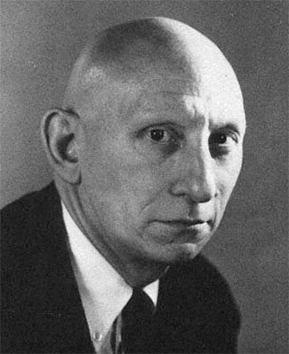
\includegraphics[width=0.50cm,height=0.55cm,keepaspectratio]{images/alanjperlis.jpg}
      };
      \node[inner sep=0pt, anchor=center] at (-2.43,1.77) {
        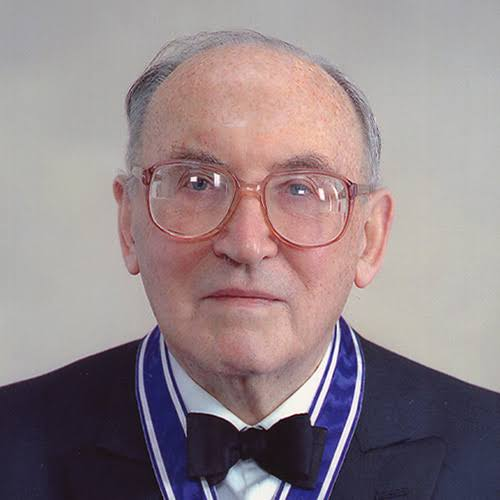
\includegraphics[width=0.50cm,height=0.55cm,keepaspectratio]{images/mauricewilkes.jpg}
      };
      \node[inner sep=0pt, anchor=center] at (-1.89,1.77) {
        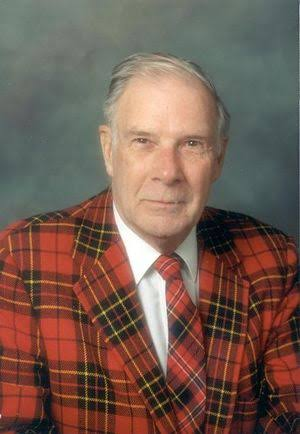
\includegraphics[width=0.50cm,height=0.55cm,keepaspectratio]{images/richardhamming.jpg}
      };
      \node[inner sep=0pt, anchor=center] at (-1.35,1.77) {
        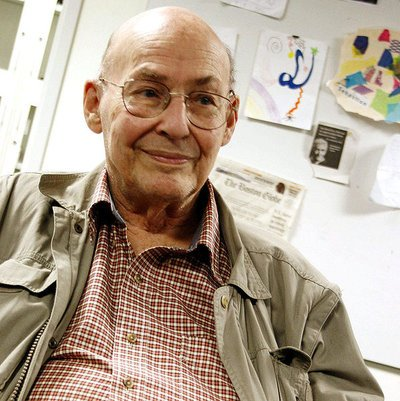
\includegraphics[width=0.50cm,height=0.55cm,keepaspectratio]{images/marvinminsky.jpg}
      };
      \node[inner sep=0pt, anchor=center] at (-0.81,1.77) {
        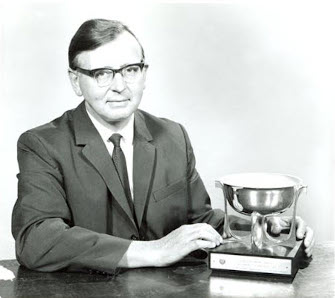
\includegraphics[width=0.50cm,height=0.55cm,keepaspectratio]{images/jameshwilkinson.jpg}
      };
      \node[inner sep=0pt, anchor=center] at (-0.27,1.77) {
        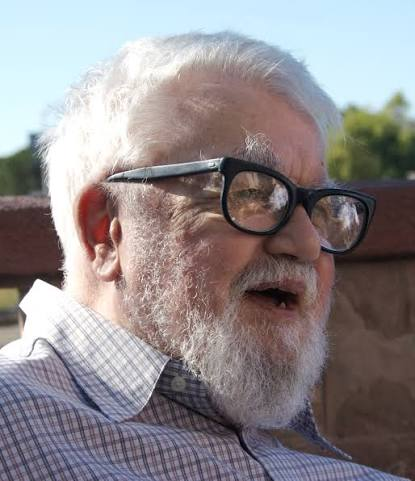
\includegraphics[width=0.50cm,height=0.55cm,keepaspectratio]{images/johnmccarthy.jpg}
      };
      \node[inner sep=0pt, anchor=center] at (0.27,1.77) {
        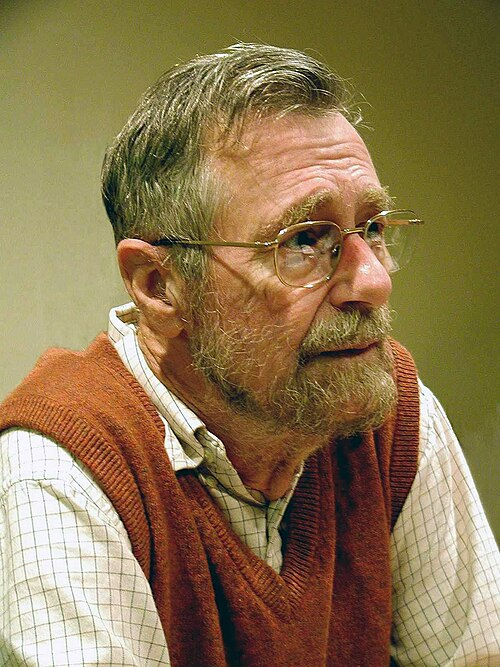
\includegraphics[width=0.50cm,height=0.55cm,keepaspectratio]{images/edsgerwdijkstra.jpg}
      };
      \node[inner sep=0pt, anchor=center] at (0.81,1.77) {
        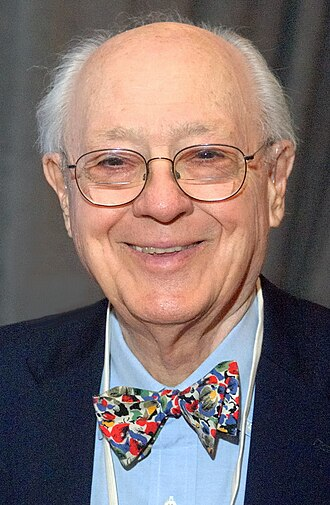
\includegraphics[width=0.50cm,height=0.55cm,keepaspectratio]{images/charlesbachman.jpg}
      };
      \node[inner sep=0pt, anchor=center] at (1.35,1.77) {
        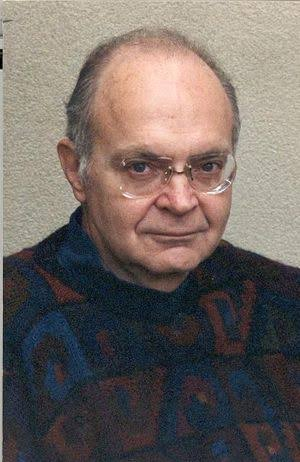
\includegraphics[width=0.50cm,height=0.55cm,keepaspectratio]{images/donaldknuth.jpg}
      };
      \node[inner sep=0pt, anchor=center] at (1.89,1.77) {
        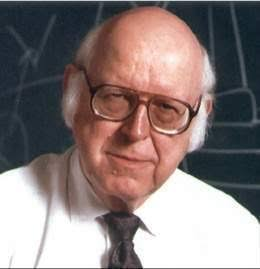
\includegraphics[width=0.50cm,height=0.55cm,keepaspectratio]{images/allennewell.jpg}
      };
      \node[inner sep=0pt, anchor=center] at (2.43,1.77) {
        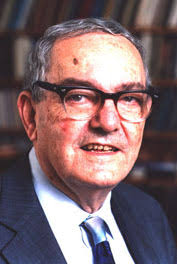
\includegraphics[width=0.50cm,height=0.55cm,keepaspectratio]{images/herbertasimon.jpg}
      };
      \node[inner sep=0pt, anchor=center] at (2.97,1.77) {
        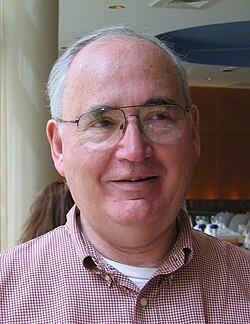
\includegraphics[width=0.50cm,height=0.55cm,keepaspectratio]{images/danascott.jpg}
      };
      \node[inner sep=0pt, anchor=center] at (-2.97,1.18) {
        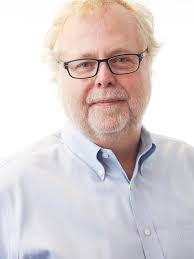
\includegraphics[width=0.50cm,height=0.55cm,keepaspectratio]{images/michaelorabin.jpg}
      };
      \node[inner sep=0pt, anchor=center] at (-2.43,1.18) {
        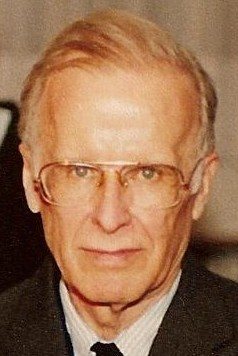
\includegraphics[width=0.50cm,height=0.55cm,keepaspectratio]{images/johnbackus.jpg}
      };
      \node[inner sep=0pt, anchor=center] at (-1.89,1.18) {
        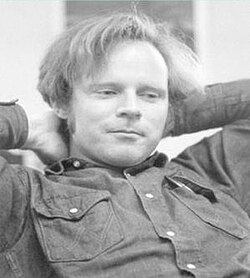
\includegraphics[width=0.50cm,height=0.55cm,keepaspectratio]{images/robertwfloyd.jpg}
      };
      \node[inner sep=0pt, anchor=center] at (-1.35,1.18) {
        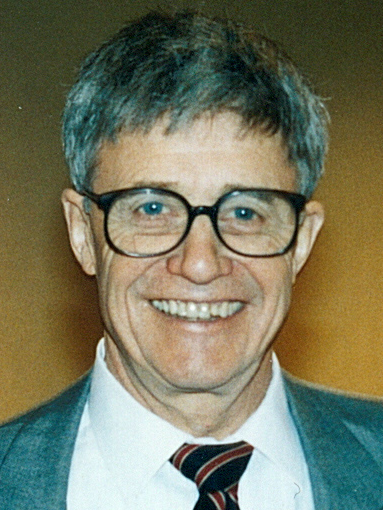
\includegraphics[width=0.50cm,height=0.55cm,keepaspectratio]{images/kennetheiverson.jpg}
      };
      \node[inner sep=0pt, anchor=center] at (-0.81,1.18) {
        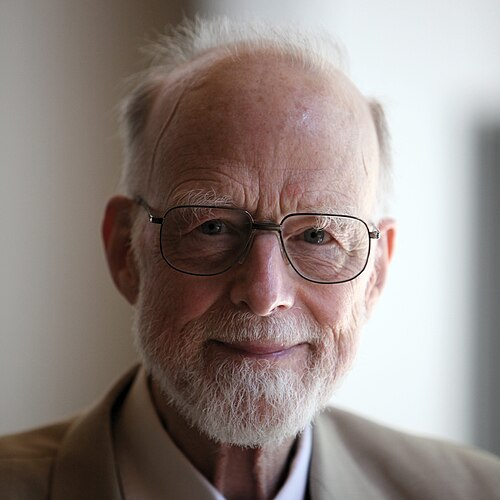
\includegraphics[width=0.50cm,height=0.55cm,keepaspectratio]{images/tonyhoare.jpg}
      };
      \node[inner sep=0pt, anchor=center] at (-0.27,1.18) {
        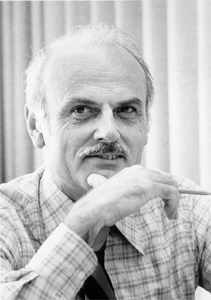
\includegraphics[width=0.50cm,height=0.55cm,keepaspectratio]{images/edgarfcodd.jpg}
      };
      \node[inner sep=0pt, anchor=center] at (0.27,1.18) {
        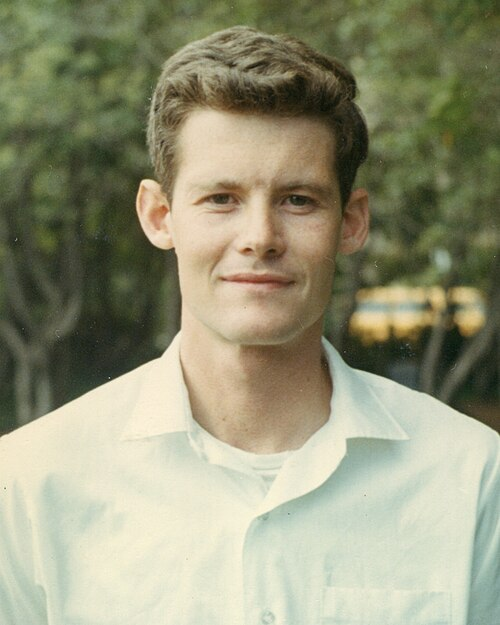
\includegraphics[width=0.50cm,height=0.55cm,keepaspectratio]{images/stephencook.jpg}
      };
      \node[inner sep=0pt, anchor=center] at (0.81,1.18) {
        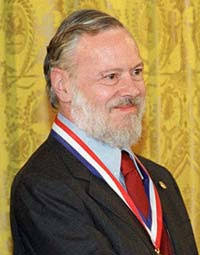
\includegraphics[width=0.50cm,height=0.55cm,keepaspectratio]{images/dennisritchie.jpg}
      };
      \node[inner sep=0pt, anchor=center] at (1.35,1.18) {
        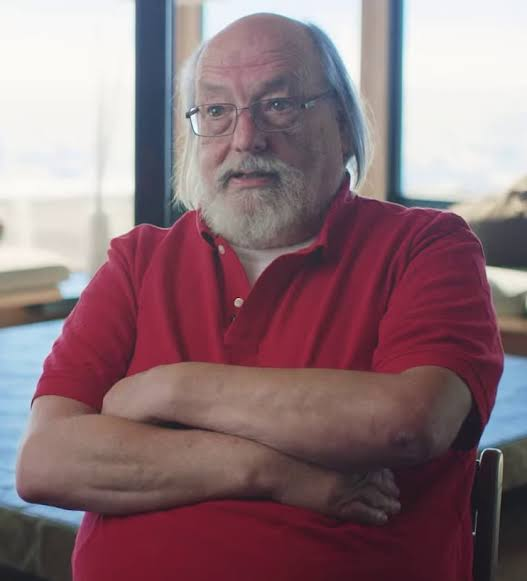
\includegraphics[width=0.50cm,height=0.55cm,keepaspectratio]{images/kenthompson.jpg}
      };
      \node[inner sep=0pt, anchor=center] at (1.89,1.18) {
        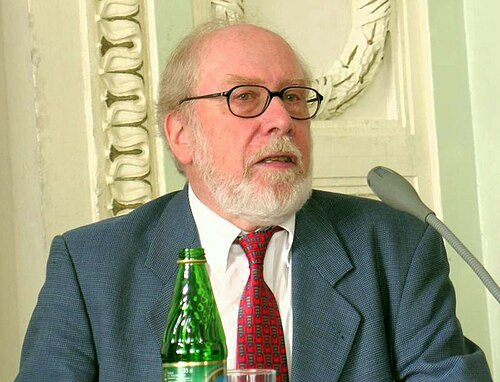
\includegraphics[width=0.50cm,height=0.55cm,keepaspectratio]{images/niklauswirth.jpg}
      };
      \node[inner sep=0pt, anchor=center] at (2.43,1.18) {
        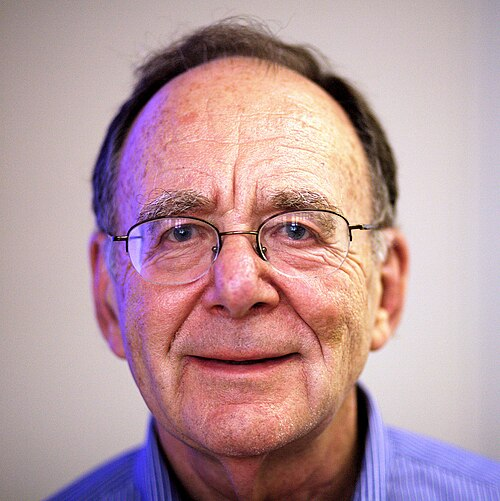
\includegraphics[width=0.50cm,height=0.55cm,keepaspectratio]{images/richardkarp.jpg}
      };
      \node[inner sep=0pt, anchor=center] at (2.97,1.18) {
        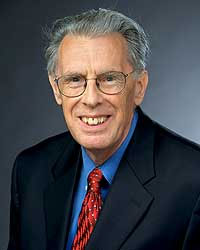
\includegraphics[width=0.50cm,height=0.55cm,keepaspectratio]{images/johnhopcroft.jpg}
      };
      \node[inner sep=0pt, anchor=center] at (-2.97,0.59) {
        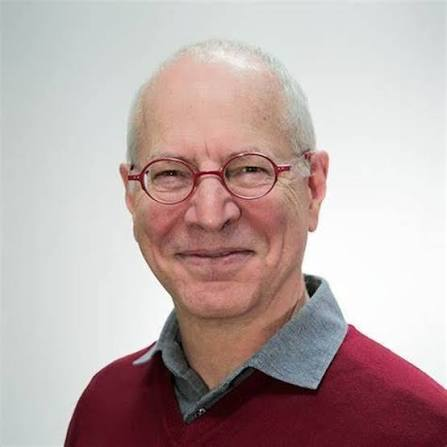
\includegraphics[width=0.50cm,height=0.55cm,keepaspectratio]{images/roberttarjan.jpg}
      };
      \node[inner sep=0pt, anchor=center] at (-2.43,0.59) {
        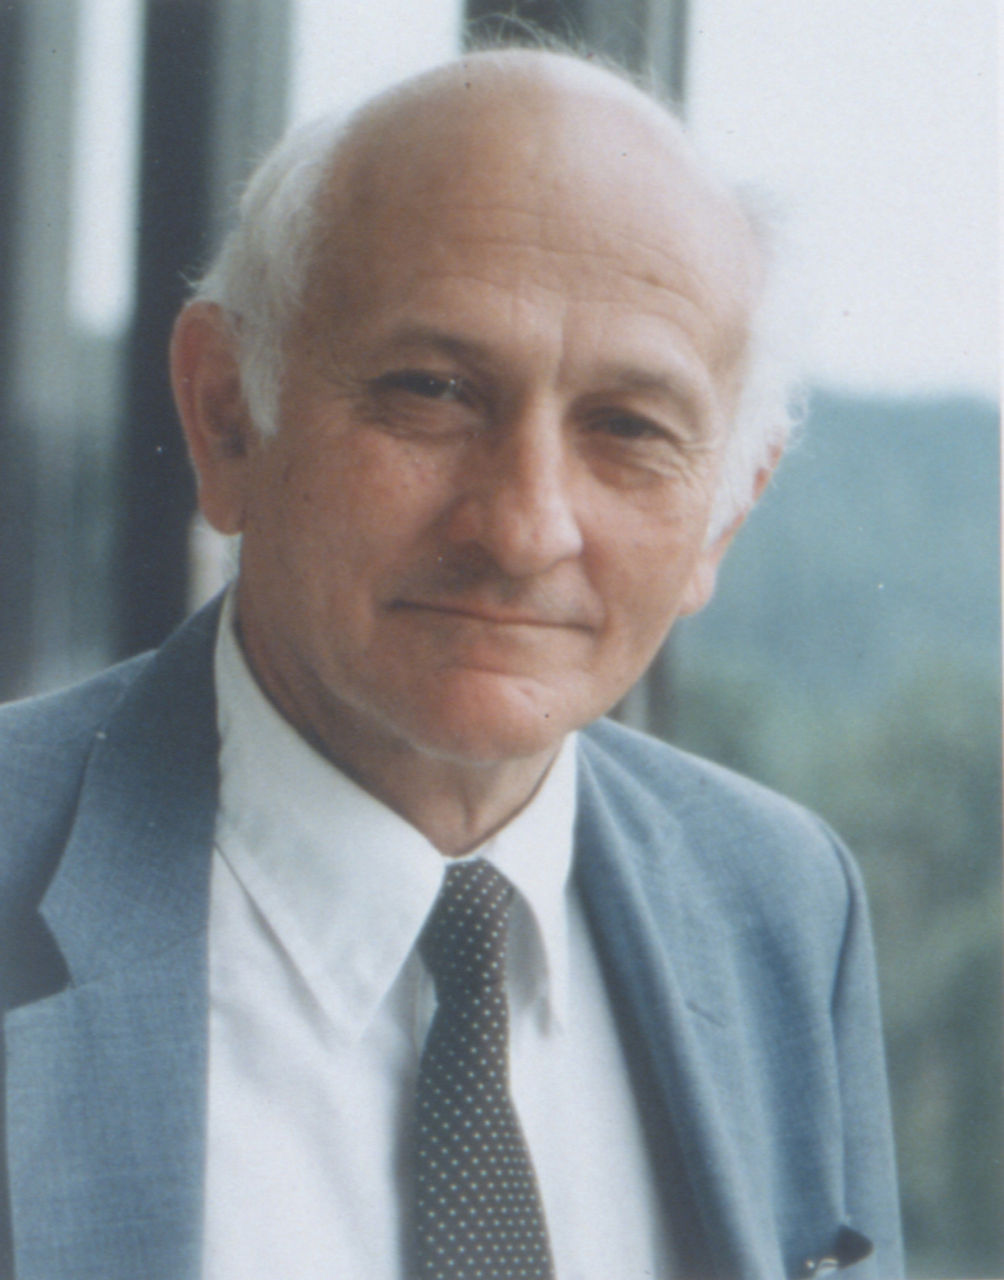
\includegraphics[width=0.50cm,height=0.55cm,keepaspectratio]{images/johncocke.jpg}
      };
      \node[inner sep=0pt, anchor=center] at (-1.89,0.59) {
        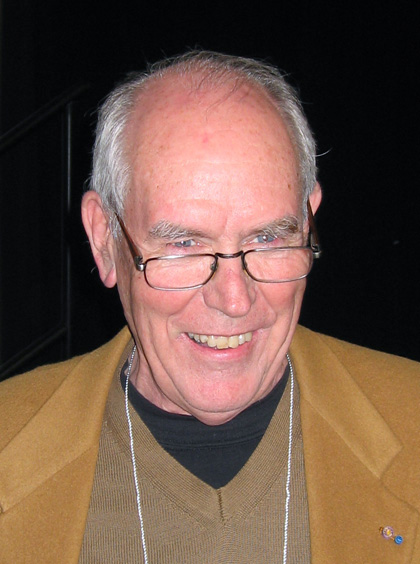
\includegraphics[width=0.50cm,height=0.55cm,keepaspectratio]{images/ivansutherland.jpg}
      };
      \node[inner sep=0pt, anchor=center] at (-1.35,0.59) {
        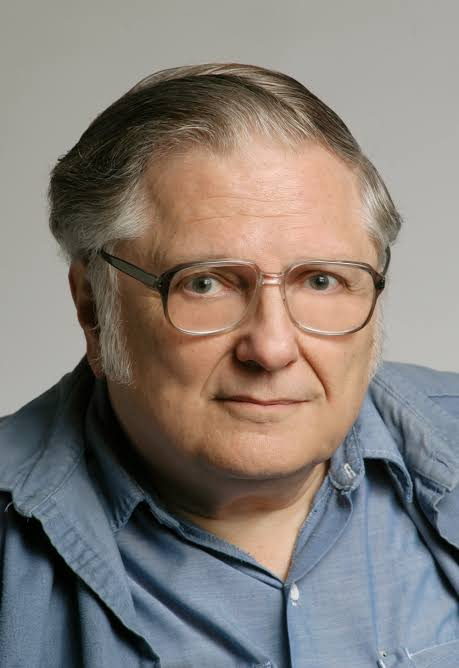
\includegraphics[width=0.50cm,height=0.55cm,keepaspectratio]{images/williamkahan.jpg}
      };
      \node[inner sep=0pt, anchor=center] at (-0.81,0.59) {
        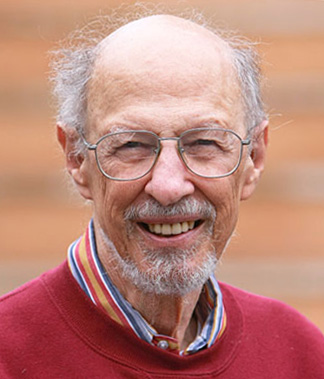
\includegraphics[width=0.50cm,height=0.55cm,keepaspectratio]{images/fernandojcorbato.jpg}
      };
      \node[inner sep=0pt, anchor=center] at (-0.27,0.59) {
        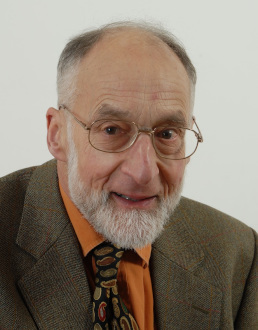
\includegraphics[width=0.50cm,height=0.55cm,keepaspectratio]{images/robinmilner.jpg}
      };
      \node[inner sep=0pt, anchor=center] at (0.27,0.59) {
        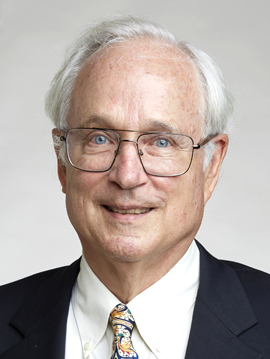
\includegraphics[width=0.50cm,height=0.55cm,keepaspectratio]{images/butlerwlampson.jpg}
      };
      \node[inner sep=0pt, anchor=center] at (0.81,0.59) {
        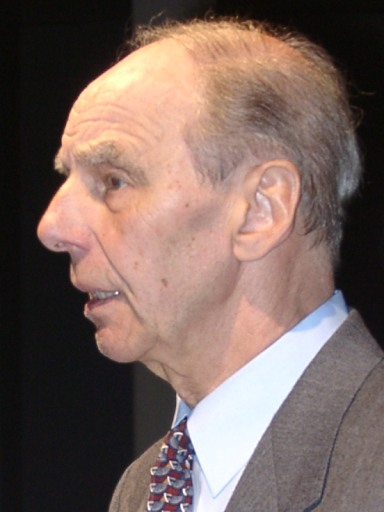
\includegraphics[width=0.50cm,height=0.55cm,keepaspectratio]{images/jurishartmanis.jpg}
      };
      \node[inner sep=0pt, anchor=center] at (1.35,0.59) {
        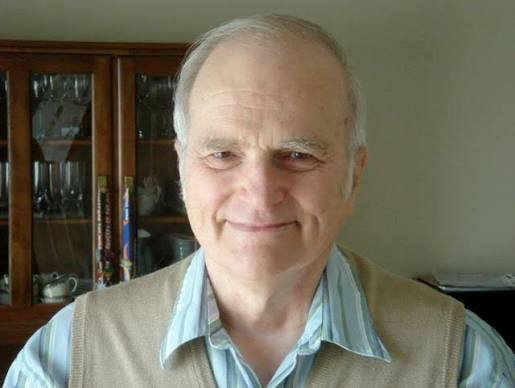
\includegraphics[width=0.50cm,height=0.55cm,keepaspectratio]{images/richardestearns.jpg}
      };
      \node[inner sep=0pt, anchor=center] at (1.89,0.59) {
        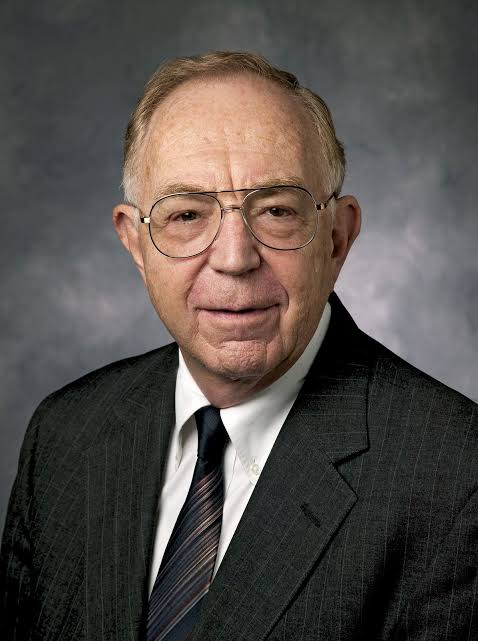
\includegraphics[width=0.50cm,height=0.55cm,keepaspectratio]{images/edwardfeigenbaum.jpg}
      };
      \node[inner sep=0pt, anchor=center] at (2.43,0.59) {
        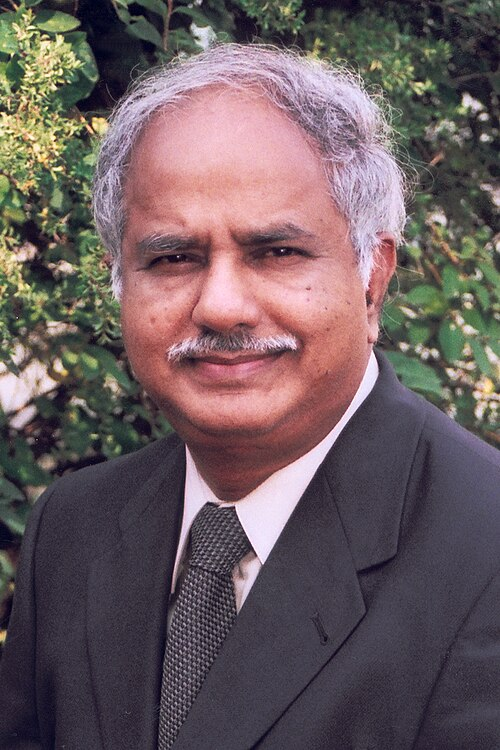
\includegraphics[width=0.50cm,height=0.55cm,keepaspectratio]{images/rajreddy.jpg}
      };
      \node[inner sep=0pt, anchor=center] at (2.97,0.59) {
        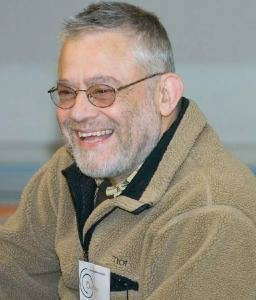
\includegraphics[width=0.50cm,height=0.55cm,keepaspectratio]{images/manuelblum.jpg}
      };
      \node[inner sep=0pt, anchor=center] at (-2.97,0.00) {
        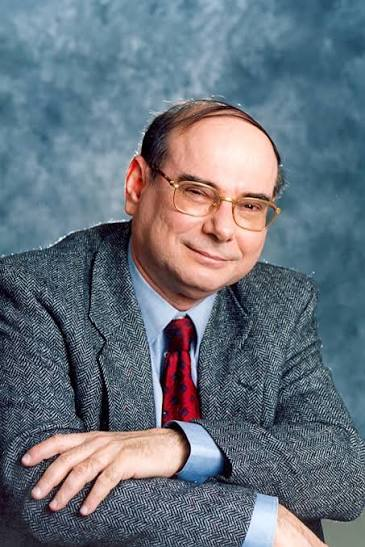
\includegraphics[width=0.50cm,height=0.55cm,keepaspectratio]{images/amirpnueli.jpg}
      };
      \node[inner sep=0pt, anchor=center] at (-2.43,0.00) {
        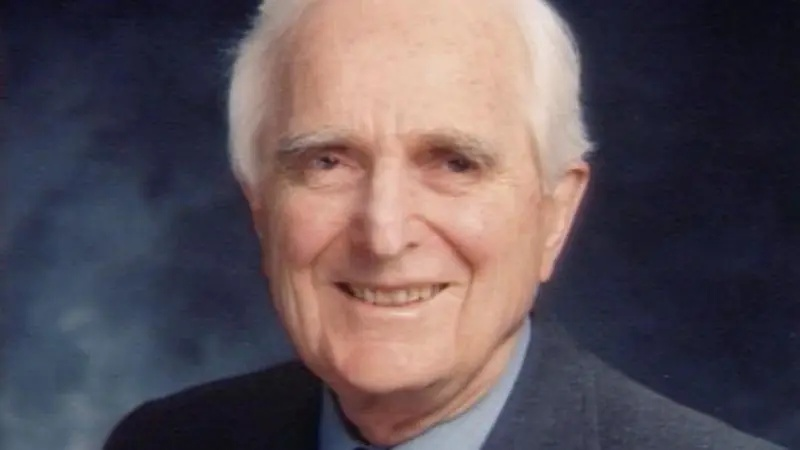
\includegraphics[width=0.50cm,height=0.55cm,keepaspectratio]{images/douglasengelbart.jpg}
      };
      \node[inner sep=0pt, anchor=center] at (-1.89,0.00) {
        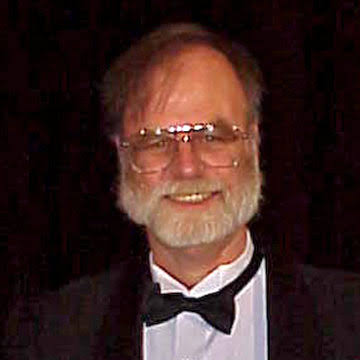
\includegraphics[width=0.50cm,height=0.55cm,keepaspectratio]{images/jimgray.jpg}
      };
      \node[inner sep=0pt, anchor=center] at (-1.35,0.00) {
        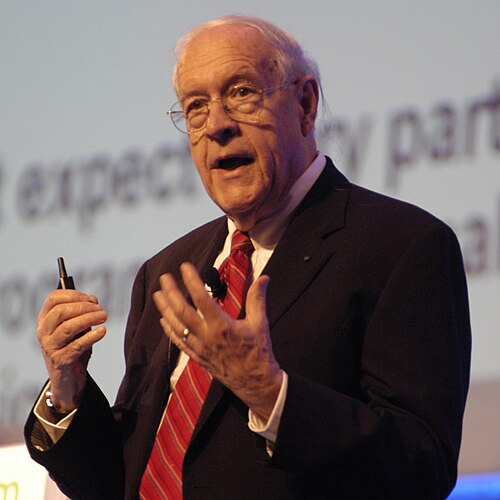
\includegraphics[width=0.50cm,height=0.55cm,keepaspectratio]{images/fredbrooks.jpg}
      };
      \node[inner sep=0pt, anchor=center] at (-0.81,0.00) {
        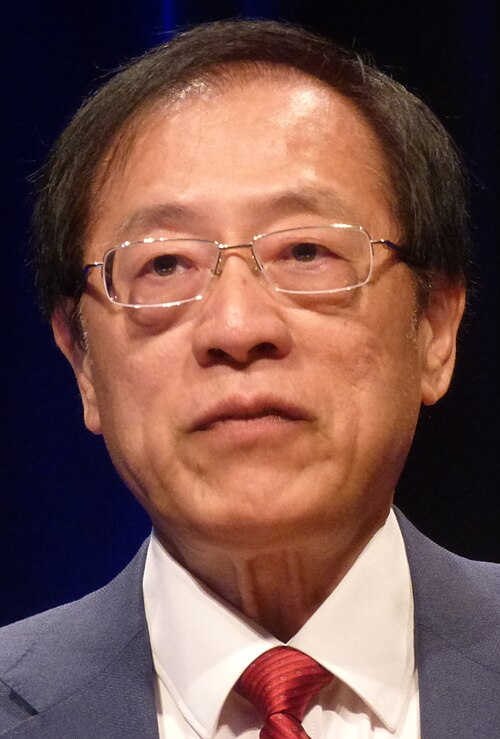
\includegraphics[width=0.50cm,height=0.55cm,keepaspectratio]{images/andrewyao.jpg}
      };
      \node[inner sep=0pt, anchor=center] at (-0.27,0.00) {
        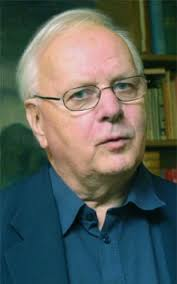
\includegraphics[width=0.50cm,height=0.55cm,keepaspectratio]{images/kristennygaard.jpg}
      };
      \node[inner sep=0pt, anchor=center] at (0.27,0.00) {
        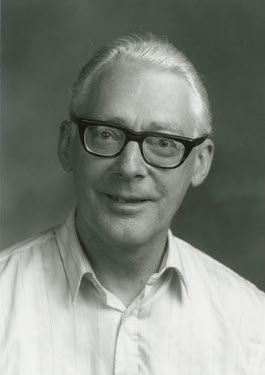
\includegraphics[width=0.50cm,height=0.55cm,keepaspectratio]{images/olejohandahl.jpg}
      };
      \node[inner sep=0pt, anchor=center] at (0.81,0.00) {
        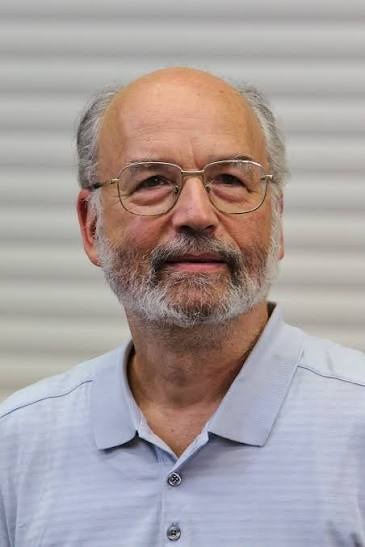
\includegraphics[width=0.50cm,height=0.55cm,keepaspectratio]{images/adishamir.jpg}
      };
      \node[inner sep=0pt, anchor=center] at (1.35,0.00) {
        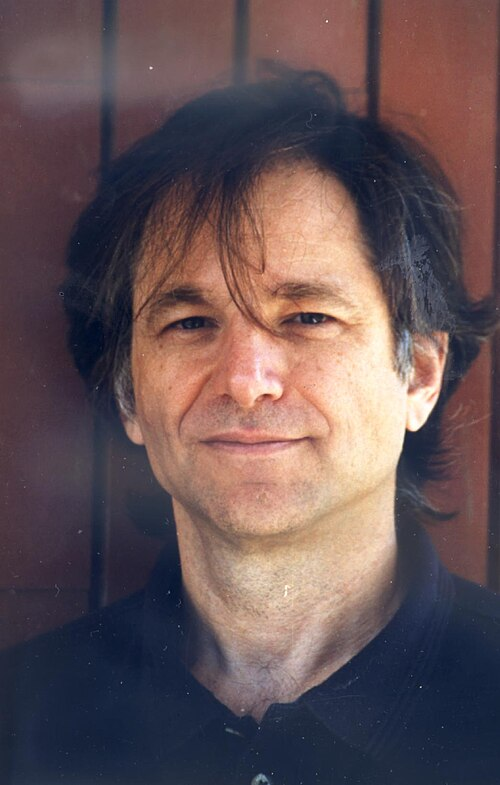
\includegraphics[width=0.50cm,height=0.55cm,keepaspectratio]{images/leonardadleman.jpg}
      };
      \node[inner sep=0pt, anchor=center] at (1.89,0.00) {
        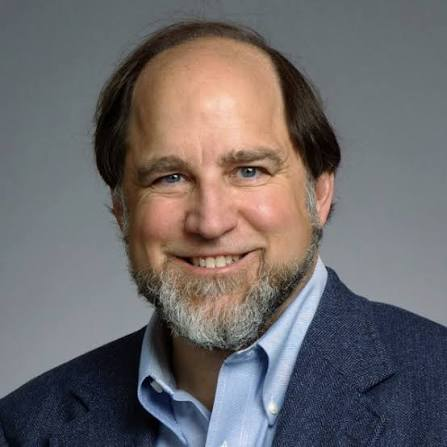
\includegraphics[width=0.50cm,height=0.55cm,keepaspectratio]{images/ronaldrivest.jpg}
      };
      \node[inner sep=0pt, anchor=center] at (2.43,0.00) {
        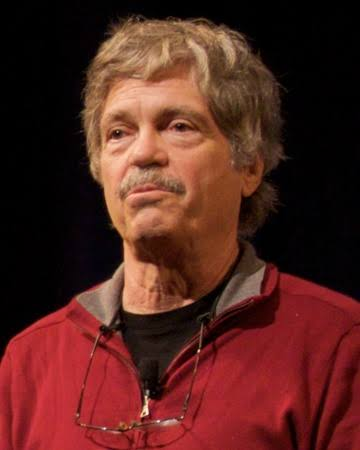
\includegraphics[width=0.50cm,height=0.55cm,keepaspectratio]{images/alankay.jpg}
      };
      \node[inner sep=0pt, anchor=center] at (2.97,0.00) {
        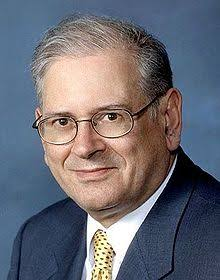
\includegraphics[width=0.50cm,height=0.55cm,keepaspectratio]{images/robertkahn.jpg}
      };
      \node[inner sep=0pt, anchor=center] at (-2.97,-0.59) {
        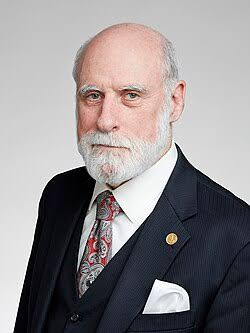
\includegraphics[width=0.50cm,height=0.55cm,keepaspectratio]{images/vintcerf.jpg}
      };
      \node[inner sep=0pt, anchor=center] at (-2.43,-0.59) {
        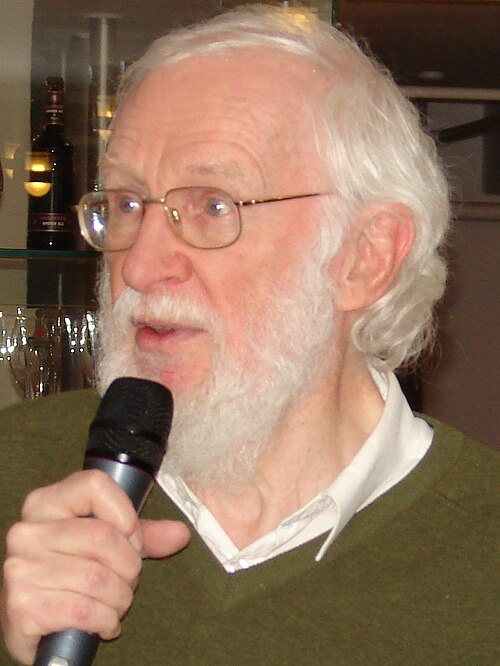
\includegraphics[width=0.50cm,height=0.55cm,keepaspectratio]{images/peternaur.jpg}
      };
      \node[inner sep=0pt, anchor=center] at (-1.89,-0.59) {
        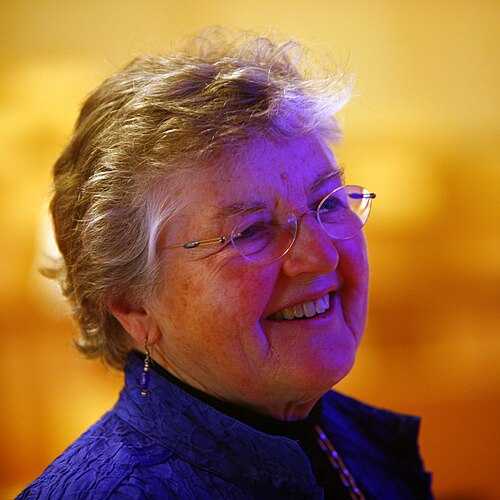
\includegraphics[width=0.50cm,height=0.55cm,keepaspectratio]{images/franceseallen.jpg}
      };
      \node[inner sep=0pt, anchor=center] at (-1.35,-0.59) {
        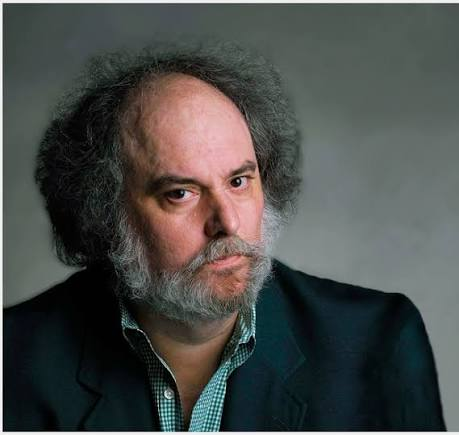
\includegraphics[width=0.50cm,height=0.55cm,keepaspectratio]{images/eallenemerson.jpg}
      };
      \node[inner sep=0pt, anchor=center] at (-0.81,-0.59) {
        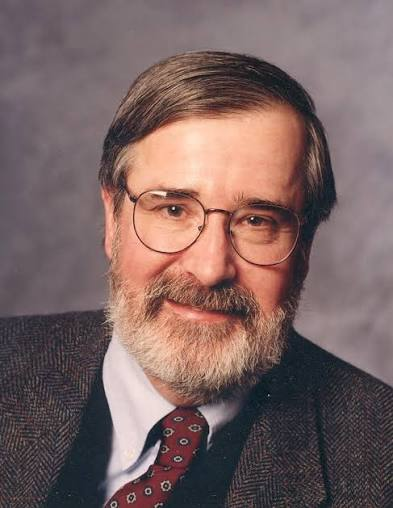
\includegraphics[width=0.50cm,height=0.55cm,keepaspectratio]{images/edmundmclarke.jpg}
      };
      \node[inner sep=0pt, anchor=center] at (-0.27,-0.59) {
        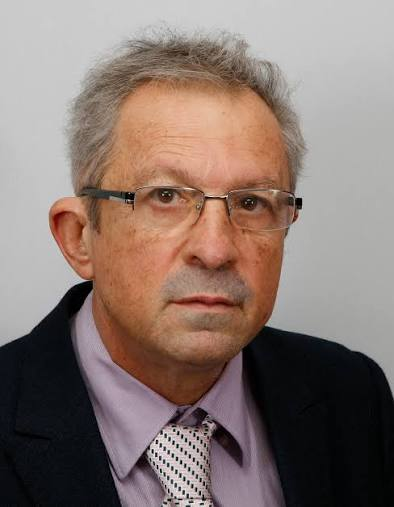
\includegraphics[width=0.50cm,height=0.55cm,keepaspectratio]{images/josephsifakis.jpg}
      };
      \node[inner sep=0pt, anchor=center] at (0.27,-0.59) {
        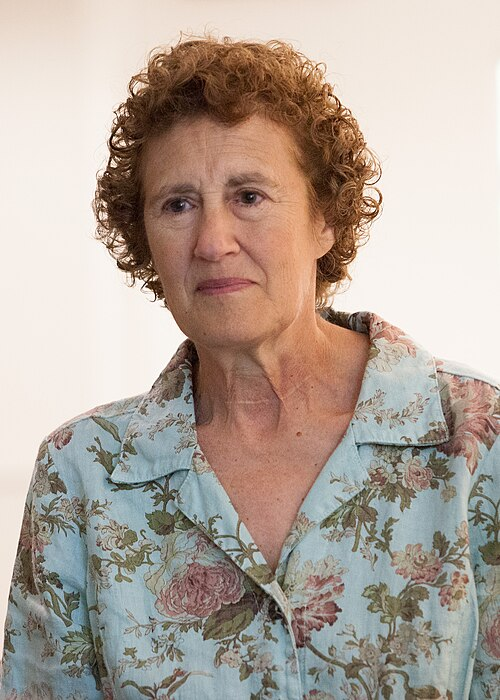
\includegraphics[width=0.50cm,height=0.55cm,keepaspectratio]{images/barbaraliskov.jpg}
      };
      \node[inner sep=0pt, anchor=center] at (0.81,-0.59) {
        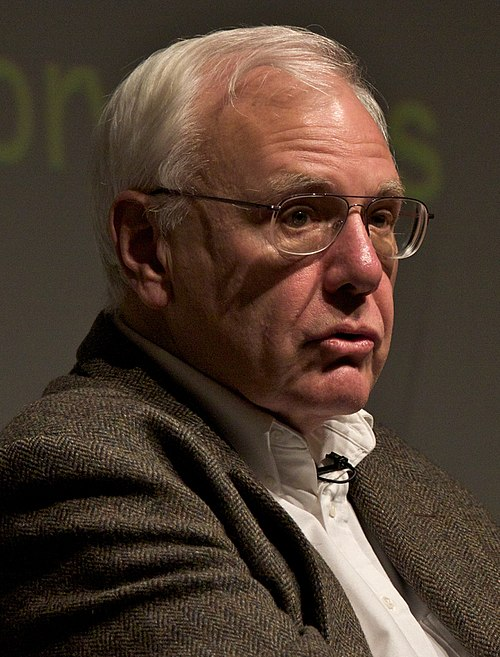
\includegraphics[width=0.50cm,height=0.55cm,keepaspectratio]{images/charlespthacker.jpg}
      };
      \node[inner sep=0pt, anchor=center] at (1.35,-0.59) {
        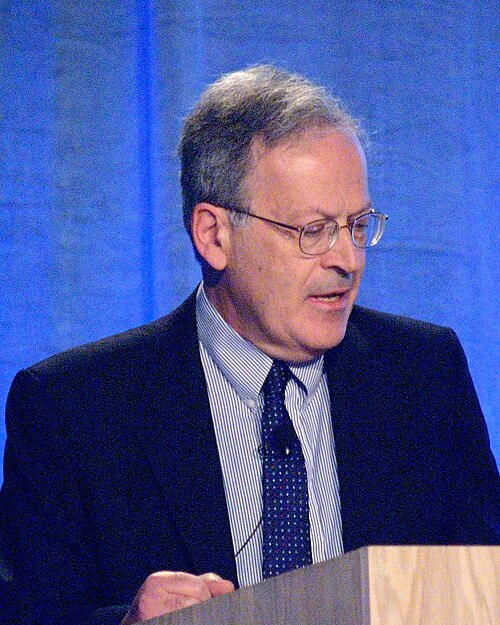
\includegraphics[width=0.50cm,height=0.55cm,keepaspectratio]{images/leslievaliant.jpg}
      };
      \node[inner sep=0pt, anchor=center] at (1.89,-0.59) {
        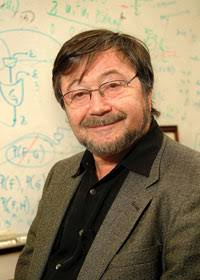
\includegraphics[width=0.50cm,height=0.55cm,keepaspectratio]{images/judeapearl.jpg}
      };
      \node[inner sep=0pt, anchor=center] at (2.43,-0.59) {
        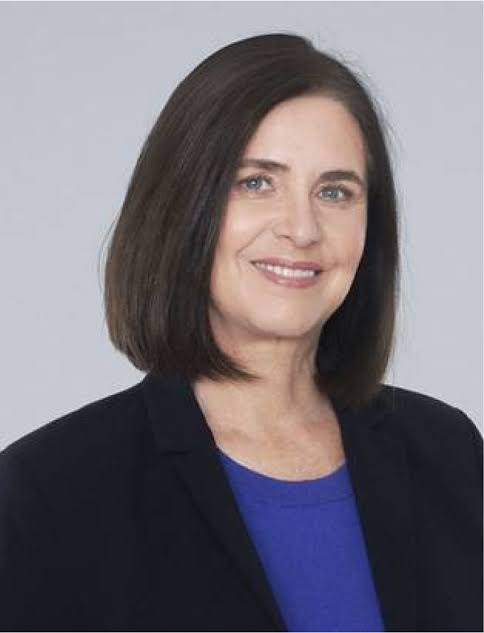
\includegraphics[width=0.50cm,height=0.55cm,keepaspectratio]{images/shafigoldwasser.jpg}
      };
      \node[inner sep=0pt, anchor=center] at (2.97,-0.59) {
        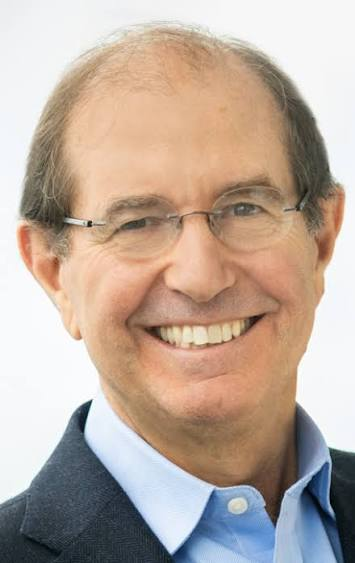
\includegraphics[width=0.50cm,height=0.55cm,keepaspectratio]{images/silviomicali.jpg}
      };
      \node[inner sep=0pt, anchor=center] at (-2.97,-1.18) {
        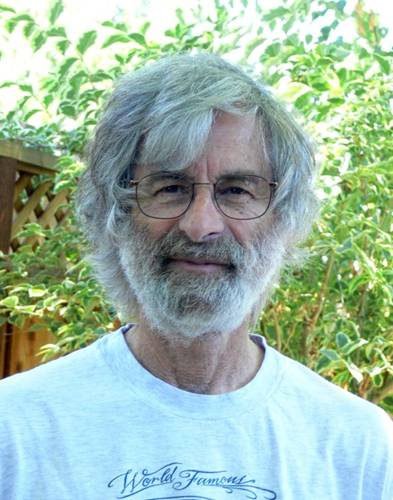
\includegraphics[width=0.50cm,height=0.55cm,keepaspectratio]{images/leslielamport.jpg}
      };
      \node[inner sep=0pt, anchor=center] at (-2.43,-1.18) {
        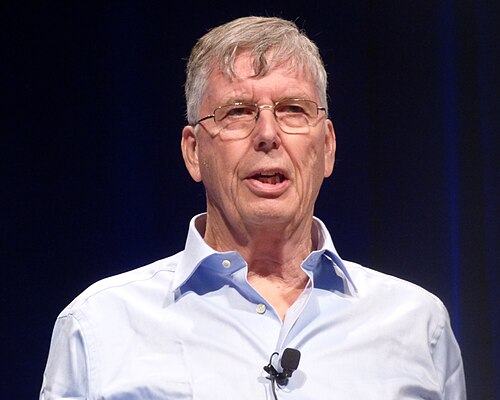
\includegraphics[width=0.50cm,height=0.55cm,keepaspectratio]{images/michaelstonebraker.jpg}
      };
      \node[inner sep=0pt, anchor=center] at (-1.89,-1.18) {
        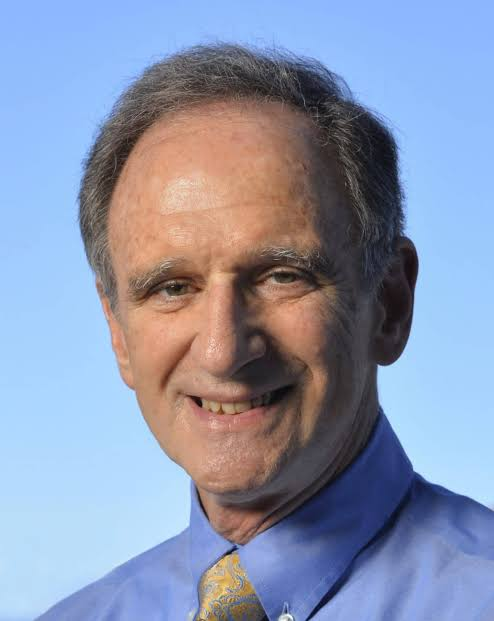
\includegraphics[width=0.50cm,height=0.55cm,keepaspectratio]{images/martinhellman.jpg}
      };
      \node[inner sep=0pt, anchor=center] at (-1.35,-1.18) {
        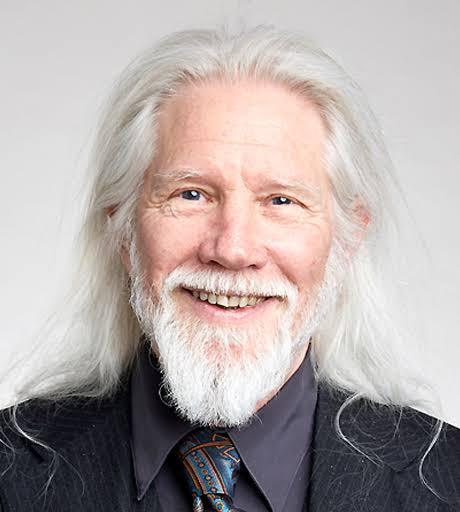
\includegraphics[width=0.50cm,height=0.55cm,keepaspectratio]{images/whitfielddiffie.jpg}
      };
      \node[inner sep=0pt, anchor=center] at (-0.81,-1.18) {
        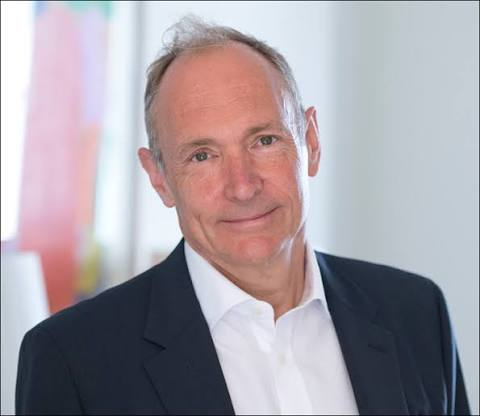
\includegraphics[width=0.50cm,height=0.55cm,keepaspectratio]{images/timbernerslee.jpg}
      };
      \node[inner sep=0pt, anchor=center] at (-0.27,-1.18) {
        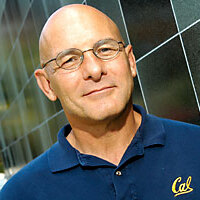
\includegraphics[width=0.50cm,height=0.55cm,keepaspectratio]{images/davidpatterson.jpg}
      };
      \node[inner sep=0pt, anchor=center] at (0.27,-1.18) {
        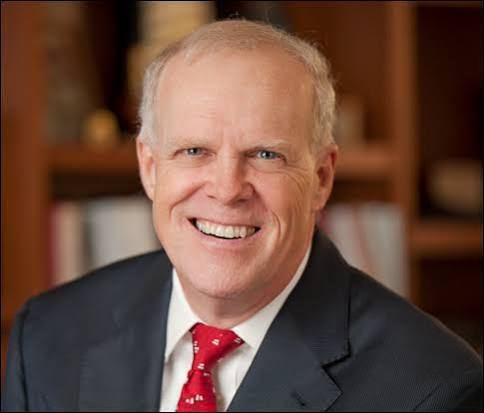
\includegraphics[width=0.50cm,height=0.55cm,keepaspectratio]{images/johnlhennessy.jpg}
      };
      \node[inner sep=0pt, anchor=center] at (0.81,-1.18) {
        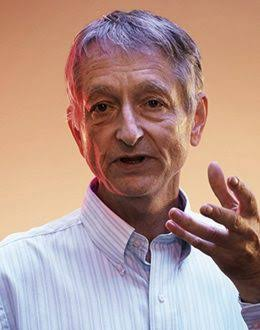
\includegraphics[width=0.50cm,height=0.55cm,keepaspectratio]{images/geoffreyhinton.jpg}
      };
      \node[inner sep=0pt, anchor=center] at (1.35,-1.18) {
        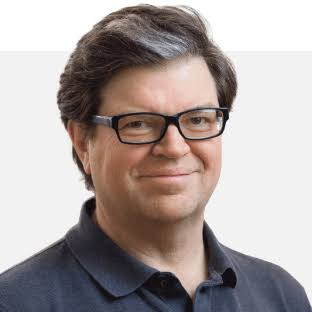
\includegraphics[width=0.50cm,height=0.55cm,keepaspectratio]{images/yannlecun.jpg}
      };
      \node[inner sep=0pt, anchor=center] at (1.89,-1.18) {
        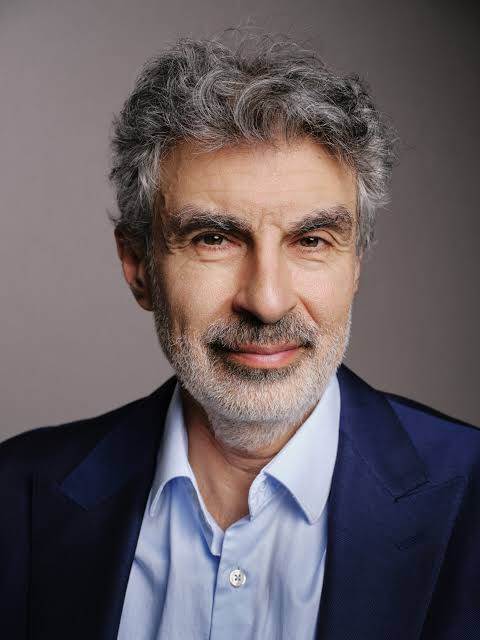
\includegraphics[width=0.50cm,height=0.55cm,keepaspectratio]{images/yoshuabengio.jpg}
      };
      \node[inner sep=0pt, anchor=center] at (2.43,-1.18) {
        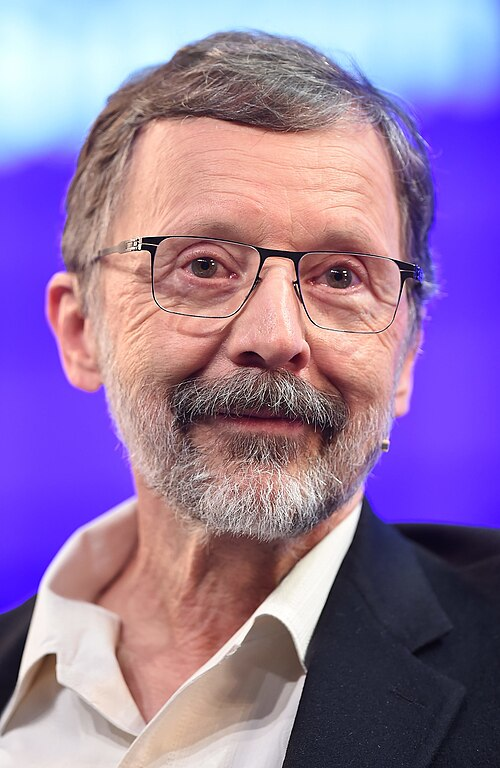
\includegraphics[width=0.50cm,height=0.55cm,keepaspectratio]{images/edwincatmull.jpg}
      };
      \node[inner sep=0pt, anchor=center] at (2.97,-1.18) {
        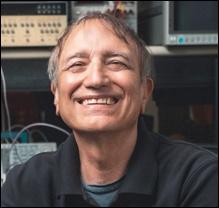
\includegraphics[width=0.50cm,height=0.55cm,keepaspectratio]{images/pathanrahan.jpg}
      };
      \node[inner sep=0pt, anchor=center] at (-2.97,-1.77) {
        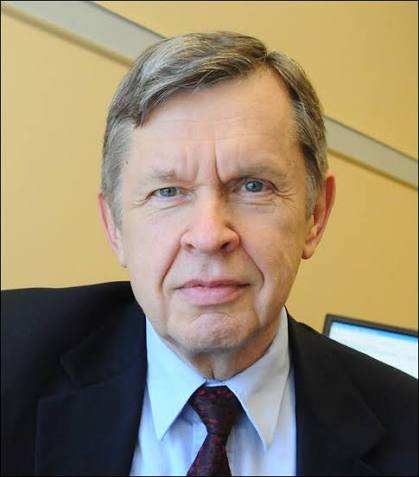
\includegraphics[width=0.50cm,height=0.55cm,keepaspectratio]{images/alfredaho.jpg}
      };
      \node[inner sep=0pt, anchor=center] at (-2.43,-1.77) {
        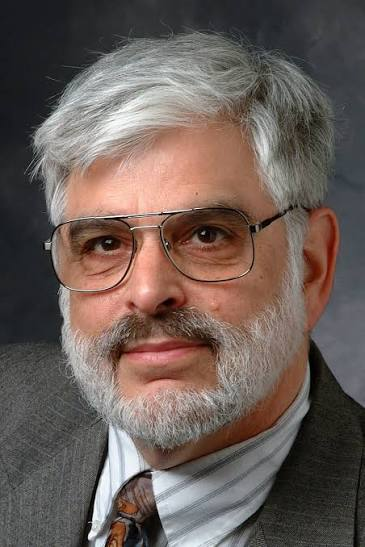
\includegraphics[width=0.50cm,height=0.55cm,keepaspectratio]{images/jeffreyullman.jpg}
      };
      \node[inner sep=0pt, anchor=center] at (-1.89,-1.77) {
        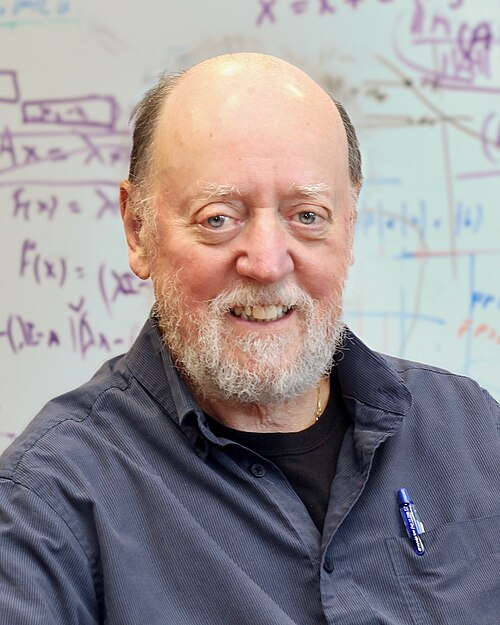
\includegraphics[width=0.50cm,height=0.55cm,keepaspectratio]{images/jackdongarra.jpg}
      };
      \node[inner sep=0pt, anchor=center] at (-1.35,-1.77) {
        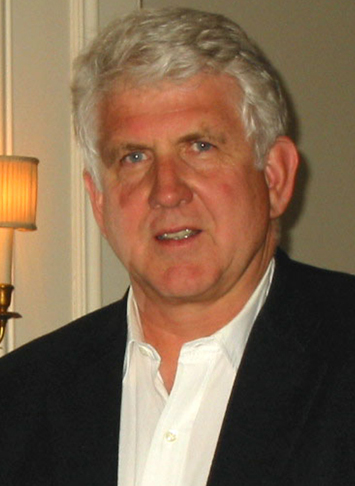
\includegraphics[width=0.50cm,height=0.55cm,keepaspectratio]{images/robertmetcalfe.jpg}
      };
      \node[inner sep=0pt, anchor=center] at (-0.81,-1.77) {
        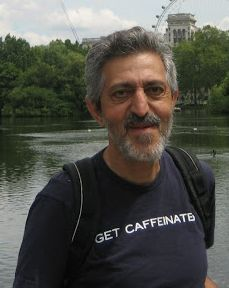
\includegraphics[width=0.50cm,height=0.55cm,keepaspectratio]{images/aviwigderson.jpg}
      };
      \node[inner sep=0pt, anchor=center] at (-0.27,-1.77) {
        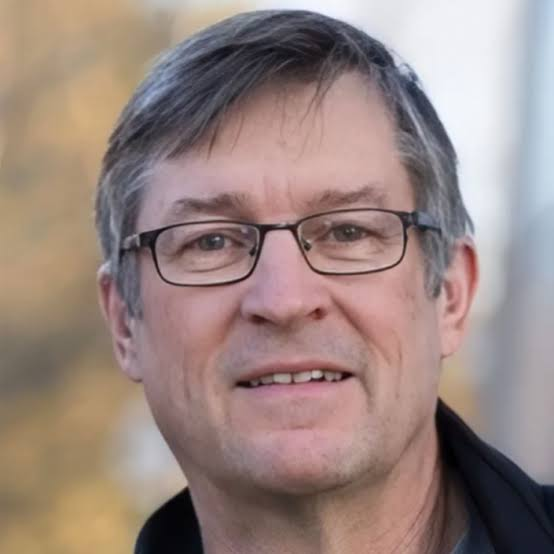
\includegraphics[width=0.50cm,height=0.55cm,keepaspectratio]{images/andrewbarto.jpg}
      };
      \node[inner sep=0pt, anchor=center] at (0.27,-1.77) {
        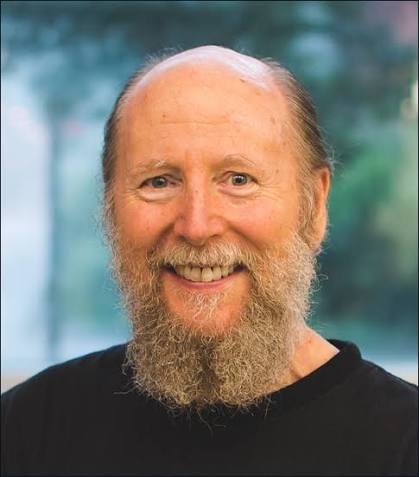
\includegraphics[width=0.50cm,height=0.55cm,keepaspectratio]{images/richardssutton.jpg}
      };
      \node[inner sep=0pt, anchor=center] at (0.81,-1.77) {
        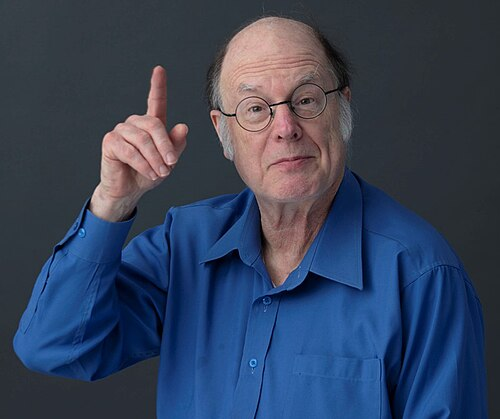
\includegraphics[width=0.50cm,height=0.55cm,keepaspectratio]{images/charleshbennett.jpg}
      };
      \node[inner sep=0pt, anchor=center] at (1.35,-1.77) {
        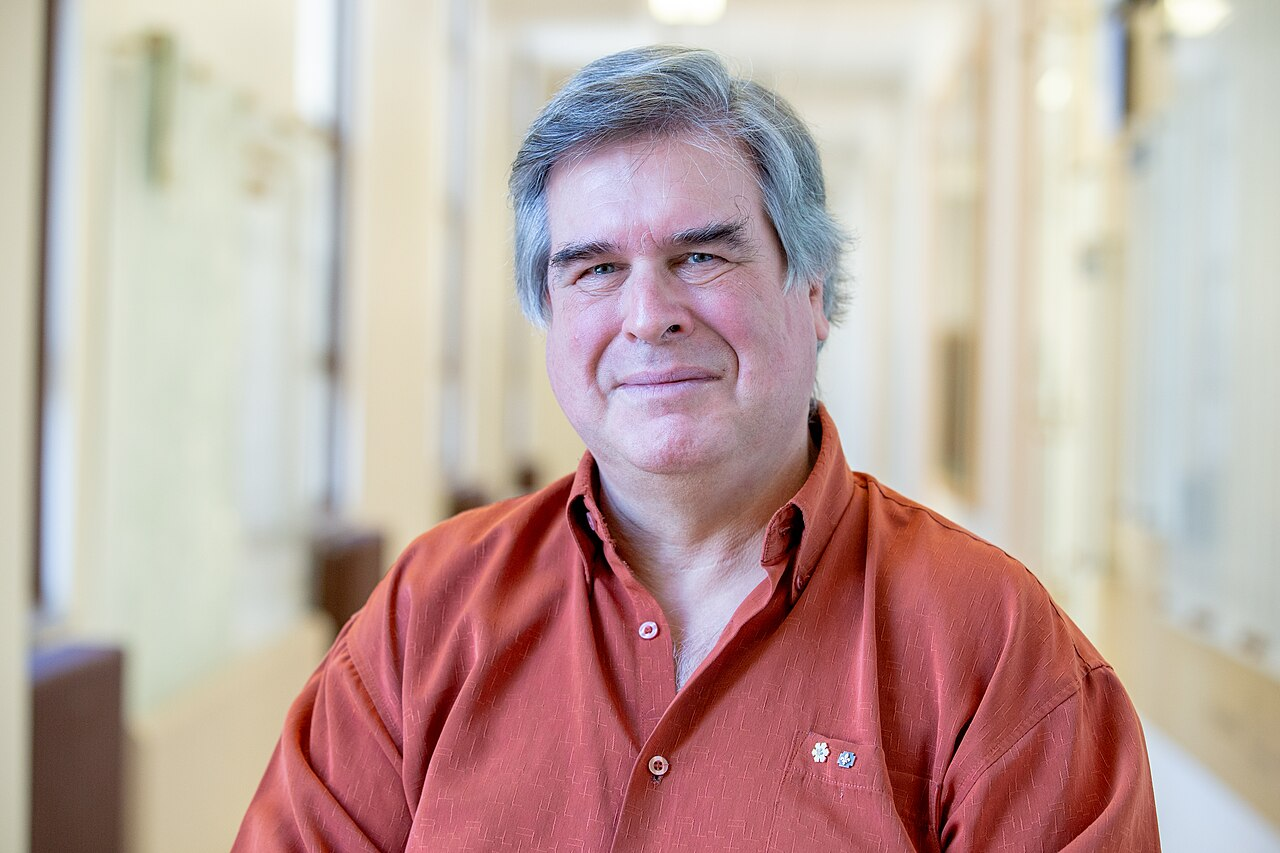
\includegraphics[width=0.50cm,height=0.55cm,keepaspectratio]{images/gillesbrassard.jpg}
      };
    \end{tikzpicture}
  };
  \node[anchor=south, font=\fontsize{6}{7}\selectfont, text=mutedgray]
    at ([yshift=0.25cm]current page.south) {\faIcon{desktop}\enspace Turing Award Laureates\enspace|\enspace ACM\enspace|\enspace 1966–2025\enspace|\enspace 60 届·81 人};
\end{tikzpicture}
\end{frame}


\def\framesubject{诺贝尔·沃尔夫·京都·哥德尔·阿贝尔·香农等顶级交叉（I）}
\begin{frame}{双料与大满贯 · 图灵奖得主身份总览}
\vspace{-4pt}
\centering
\begin{tikzpicture}
  \node[fill=nsmclr, rounded corners=4pt, text width=3.5cm, minimum height=0.55cm,
        inner sep=0pt, align=center, anchor=north west] at (-5.4,0.00)
    {\fontsize{5.5}{6.5}\selectfont\bfseries\color{white}$\spadesuit$\;\; 美国国家科学奖章\;\; 9人};
  \node[anchor=north west, text width=8.0cm, align=left,
        font=\fontsize{5.5}{6.5}\selectfont, text=nsmclr!70!black]
    at (-1.70,0.00) {John McCarthy\;·\;Donald Knuth\;·\;Herbert A. Simon\;·\;John Backus\;·\;Richard Karp \\ William Kahan\;·\;Judea Pearl\;·\;Yann LeCun\;·\;Jack Dongarra};
  \node[fill=kyotoclr, rounded corners=4pt, text width=3.5cm, minimum height=0.55cm,
        inner sep=0pt, align=center, anchor=north west] at (-5.4,-0.55)
    {\fontsize{5.5}{6.5}\selectfont\bfseries\color{white}$\blacklozenge$\;\; 京都奖\;\; 7人};
  \node[anchor=north west, text width=8.0cm, align=left,
        font=\fontsize{5.5}{6.5}\selectfont, text=kyotoclr!70!black]
    at (-1.70,-0.55) {John McCarthy\;·\;Donald Knuth\;·\;Tony Hoare\;·\;Richard Karp\;·\;Ivan Sutherland \\ Andrew Yao\;·\;Alan Kay};
  \node[fill=frsclr, rounded corners=4pt, text width=3.5cm, minimum height=0.55cm,
        inner sep=0pt, align=center, anchor=north west] at (-5.4,-1.10)
    {\fontsize{5.5}{6.5}\selectfont\bfseries\color{white}$\checkmark$\;\; 英国皇家学会院士\;\; 7人};
  \node[anchor=north west, text width=8.0cm, align=left,
        font=\fontsize{5.5}{6.5}\selectfont, text=frsclr!70!black]
    at (-1.70,-1.10) {Adi Shamir\;·\;Whitfield Diffie\;·\;Tim Berners-Lee\;·\;Geoffrey Hinton\;·\;Yoshua Bengio \\ Jack Dongarra\;·\;Gilles Brassard};
  \node[fill=marconiclr, rounded corners=4pt, text width=3.5cm, minimum height=0.55cm,
        inner sep=0pt, align=center, anchor=north west] at (-5.4,-1.65)
    {\fontsize{5.5}{6.5}\selectfont\bfseries\color{white}$\bullet$\;\; 马可尼奖\;\; 5人};
  \node[anchor=north west, text width=8.0cm, align=left,
        font=\fontsize{5.5}{6.5}\selectfont, text=marconiclr!70!black]
    at (-1.70,-1.65) {Ronald Rivest\;·\;Vint Cerf\;·\;Martin Hellman\;·\;Whitfield Diffie\;·\;Robert Metcalfe};
  \node[fill=nasclr, rounded corners=4pt, text width=3.5cm, minimum height=0.55cm,
        inner sep=0pt, align=center, anchor=north west] at (-5.4,-2.20)
    {\fontsize{5.5}{6.5}\selectfont\bfseries\color{white}$\blacksquare$\;\; 美国科学院院士\;\; 5人};
  \node[anchor=north west, text width=8.0cm, align=left,
        font=\fontsize{5.5}{6.5}\selectfont, text=nasclr!70!black]
    at (-1.70,-2.20) {Shafi Goldwasser\;·\;Silvio Micali\;·\;Leslie Lamport\;·\;Tim Berners-Lee\;·\;Yann LeCun};
  \node[fill=japanclr, rounded corners=4pt, text width=3.5cm, minimum height=0.55cm,
        inner sep=0pt, align=center, anchor=north west] at (-5.4,-2.75)
    {\fontsize{5.5}{6.5}\selectfont\bfseries\color{white}$\heartsuit$\;\; 日本国际奖\;\; 4人};
  \node[anchor=north west, text width=8.0cm, align=left,
        font=\fontsize{5.5}{6.5}\selectfont, text=japanclr!70!black]
    at (-1.70,-2.75) {Marvin Minsky\;·\;Dennis Ritchie\;·\;Ken Thompson\;·\;Vint Cerf};
  \node[fill=neumannclr, rounded corners=4pt, text width=3.5cm, minimum height=0.55cm,
        inner sep=0pt, align=center, anchor=north west] at (-5.4,-3.30)
    {\fontsize{5.5}{6.5}\selectfont\bfseries\color{white}$\blacktriangle$\;\; IEEE 冯·诺依曼奖\;\; 4人};
  \node[anchor=north west, text width=8.0cm, align=left,
        font=\fontsize{5.5}{6.5}\selectfont, text=neumannclr!70!black]
    at (-1.70,-3.30) {Tony Hoare\;·\;Ivan Sutherland\;·\;Barbara Liskov\;·\;Leslie Lamport};
  \node[fill=ntmclr, rounded corners=4pt, text width=3.5cm, minimum height=0.55cm,
        inner sep=0pt, align=center, anchor=north west] at (-5.4,-3.85)
    {\fontsize{5.5}{6.5}\selectfont\bfseries\color{white}$\star$\;\; 美国国家技术奖章\;\; 4人};
  \node[anchor=north west, text width=8.0cm, align=left,
        font=\fontsize{5.5}{6.5}\selectfont, text=ntmclr!70!black]
    at (-1.70,-3.85) {Dennis Ritchie\;·\;Ken Thompson\;·\;Vint Cerf\;·\;Robert Metcalfe};
  \fill[turingbg, rounded corners=4pt] (-5.5,-5.30) rectangle (5.6,-4.80);
  \node[anchor=north, text width=3.7cm, align=center,
               font=\fontsize{4.5}{5.5}\selectfont\bfseries, text=turingclr]
    at (-3.60,-4.90) {首届\;\; Alan J. Perlis\;(1966)};
  \node[anchor=north, text width=3.7cm, align=center,
               font=\fontsize{4.5}{5.5}\selectfont\bfseries, text=turingclr]
    at (0.00,-4.90) {60 届\;\; 81 位得主};
  \node[anchor=north, text width=3.7cm, align=center,
               font=\fontsize{4.5}{5.5}\selectfont\bfseries, text=turingclr]
    at (3.60,-4.90) {图灵+沃尔夫\;\; Shamir·Bennett·Brassard};
\end{tikzpicture}
\end{frame}

\def\framesubject{哥德尔·诺贝尔·EATCS·内万林纳等其它荣誉（II）}
\begin{frame}{双料与大满贯 · 图灵奖得主身份总览}
\vspace{-4pt}
\centering
\begin{tikzpicture}
  \node[fill=hammingclr, rounded corners=4pt, text width=3.5cm, minimum height=0.55cm,
        inner sep=0pt, align=center, anchor=north west] at (-5.4,0.00)
    {\fontsize{5.5}{6.5}\selectfont\bfseries\color{white}$\bigstar$\;\; IEEE 汉明奖章\;\; 3人};
  \node[anchor=north west, text width=8.0cm, align=left,
        font=\fontsize{5.5}{6.5}\selectfont, text=hammingclr!70!black]
    at (-1.70,0.00) {Richard Hamming\;·\;Martin Hellman\;·\;Whitfield Diffie};
  \node[fill=wolfclr, rounded corners=4pt, text width=3.5cm, minimum height=0.55cm,
        inner sep=0pt, align=center, anchor=north west] at (-5.4,-0.55)
    {\fontsize{5.5}{6.5}\selectfont\bfseries\color{white}$\bigstar$\;\; 沃尔夫奖\;\; 3人};
  \node[anchor=north west, text width=8.0cm, align=left,
        font=\fontsize{5.5}{6.5}\selectfont, text=wolfclr!70!black]
    at (-1.70,-0.55) {Adi Shamir\;·\;Charles H. Bennett\;·\;Gilles Brassard};
  \node[fill=godelclr, rounded corners=4pt, text width=3.5cm, minimum height=0.55cm,
        inner sep=0pt, align=center, anchor=north west] at (-5.4,-1.10)
    {\fontsize{5.5}{6.5}\selectfont\bfseries\color{white}$\diamond$\;\; 哥德尔奖\;\; 3人};
  \node[anchor=north west, text width=8.0cm, align=left,
        font=\fontsize{5.5}{6.5}\selectfont, text=godelclr!70!black]
    at (-1.70,-1.10) {Shafi Goldwasser\;·\;Silvio Micali\;·\;Avi Wigderson};
  \node[fill=nobelclr, rounded corners=4pt, text width=3.5cm, minimum height=0.55cm,
        inner sep=0pt, align=center, anchor=north west] at (-5.4,-1.65)
    {\fontsize{5.5}{6.5}\selectfont\bfseries\color{white}\faIcon{award}\;\; 诺贝尔奖\;\; 2人};
  \node[anchor=north west, text width=8.0cm, align=left,
        font=\fontsize{5.5}{6.5}\selectfont, text=nobelclr!70!black]
    at (-1.70,-1.65) {Herbert A. Simon\;·\;Geoffrey Hinton};
  \node[fill=eatcsclr, rounded corners=4pt, text width=3.5cm, minimum height=0.55cm,
        inner sep=0pt, align=center, anchor=north west] at (-5.4,-2.20)
    {\fontsize{5.5}{6.5}\selectfont\bfseries\color{white}$\square$\;\; EATCS 奖\;\; 2人};
  \node[anchor=north west, text width=8.0cm, align=left,
        font=\fontsize{5.5}{6.5}\selectfont, text=eatcsclr!70!black]
    at (-1.70,-2.20) {Richard Karp\;·\;Leslie Valiant};
  \node[fill=nevanclr, rounded corners=4pt, text width=3.5cm, minimum height=0.55cm,
        inner sep=0pt, align=center, anchor=north west] at (-5.4,-2.75)
    {\fontsize{5.5}{6.5}\selectfont\bfseries\color{white}$\blacktriangle$\;\; 内万林纳奖\;\; 2人};
  \node[anchor=north west, text width=8.0cm, align=left,
        font=\fontsize{5.5}{6.5}\selectfont, text=nevanclr!70!black]
    at (-1.70,-2.75) {Leslie Valiant\;·\;Avi Wigderson};
  \node[fill=rumelclr, rounded corners=4pt, text width=3.5cm, minimum height=0.55cm,
        inner sep=0pt, align=center, anchor=north west] at (-5.4,-3.30)
    {\fontsize{5.5}{6.5}\selectfont\bfseries\color{white}$\diamondsuit$\;\; 鲁梅哈特奖\;\; 1人};
  \node[anchor=north west, text width=8.0cm, align=left,
        font=\fontsize{5.5}{6.5}\selectfont, text=rumelclr!70!black]
    at (-1.70,-3.30) {Judea Pearl};
  \node[fill=abelclr, rounded corners=4pt, text width=3.5cm, minimum height=0.55cm,
        inner sep=0pt, align=center, anchor=north west] at (-5.4,-3.85)
    {\fontsize{5.5}{6.5}\selectfont\bfseries\color{white}$\bigstar$\;\; 阿贝尔奖\;\; 1人};
  \node[anchor=north west, text width=8.0cm, align=left,
        font=\fontsize{5.5}{6.5}\selectfont, text=abelclr!70!black]
    at (-1.70,-3.85) {Avi Wigderson};
  \node[fill=shannonclr, rounded corners=4pt, text width=3.5cm, minimum height=0.55cm,
        inner sep=0pt, align=center, anchor=north west] at (-5.4,-4.40)
    {\fontsize{5.5}{6.5}\selectfont\bfseries\color{white}$\bigstar$\;\; IEEE 香农奖\;\; 1人};
  \node[anchor=north west, text width=8.0cm, align=left,
        font=\fontsize{5.5}{6.5}\selectfont, text=shannonclr!70!black]
    at (-1.70,-4.40) {Charles H. Bennett};
  \fill[turingbg, rounded corners=4pt] (-5.5,-5.85) rectangle (5.6,-5.35);
  \node[anchor=north, text width=3.7cm, align=center,
               font=\fontsize{4.5}{5.5}\selectfont\bfseries, text=turingclr]
    at (-3.60,-5.45) {图灵+诺奖\;\; Simon·Hinton};
  \node[anchor=north, text width=3.7cm, align=center,
               font=\fontsize{4.5}{5.5}\selectfont\bfseries, text=turingclr]
    at (0.00,-5.45) {图灵+哥德尔\;\; Goldwasser·Micali·Wigderson};
  \node[anchor=north, text width=3.7cm, align=center,
               font=\fontsize{4.5}{5.5}\selectfont\bfseries, text=turingclr]
    at (3.60,-5.45) {图灵+哥德尔+阿贝尔\;\; Wigderson};
\end{tikzpicture}
\end{frame}


\def\framesubject{首届得主·EDSAC 存储程序计算机、·数值方法、纠错码（汉明码）·人工智能奠基人·数值分析、舍入误差分析}
\begin{frame}{1966–1970}
\vspace{-2pt}
\centering
\scriptsize
\begin{tabular}{@{}
  >{\raggedright}m{2.5cm}
  >{\centering}m{1.0cm}
  >{\centering}m{1.95cm}
  >{\raggedleft}m{1.5cm}
  >{\raggedright}m{2.2cm}
  >{\raggedright\arraybackslash}m{2.35cm}
@{}}
\toprule
\rowcolor{turingbg}
\textbf{姓名} & \textbf{获奖年份} & \textbf{生卒} & \textbf{国籍} & \textbf{机构} & \textbf{研究领域} \\
\midrule
  \lrow{Alan J. Perlis\cn{艾伦·佩利斯}}{1966}{1922–1990(享年68)}{美国}{Carnegie Mellon University}{首届得主，Algol 语言与编译技术先驱。}
  \lrow{Maurice Wilkes\cn{莫里斯·威尔克斯}}{1967}{1913–2010(享年97)}{英国}{University of Cambridge}{EDSAC 存储程序计算机、微程序设计。}
  \lrow{Richard Hamming\hammingbadge\cn{理查德·汉明}}{1968}{1915–1998(享年83)}{美国}{Bell Labs}{数值方法、纠错码（汉明码），信息论先驱。}
  \lrow{Marvin Minsky\japanbadge\cn{马文·明斯基}}{1969}{1927–2016(享年89)}{美国}{MIT}{人工智能奠基人，框架理论、神经网络早期研究。}
  \lrow{James H. Wilkinson\cn{詹姆斯·威尔金森}}{1970}{1919–1986(享年67)}{英国}{National Physical Laboratory}{数值分析、舍入误差分析，线性代数数值算法。}
\bottomrule
\end{tabular}
\vspace{6pt}
  {\centering
  \begin{tikzpicture}
      \node[inner sep=0pt] at (-3.00,0) {
        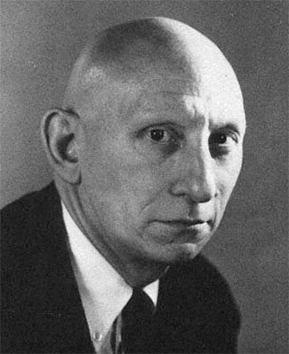
\includegraphics[width=1.80cm,height=2.20cm,keepaspectratio]{images/alanjperlis.jpg}
      };
      \node[inner sep=0pt] at (-1.50,0) {
        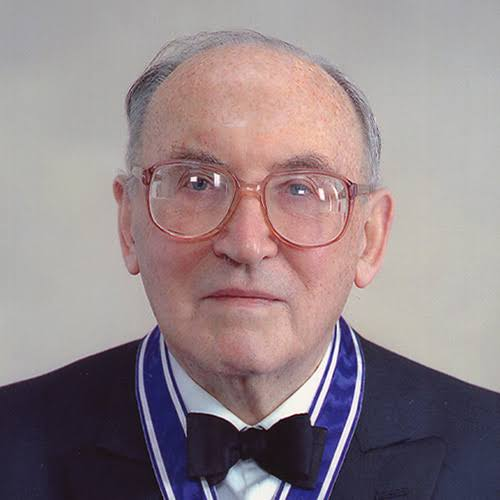
\includegraphics[width=1.80cm,height=2.20cm,keepaspectratio]{images/mauricewilkes.jpg}
      };
      \node[inner sep=0pt] at (0.00,0) {
        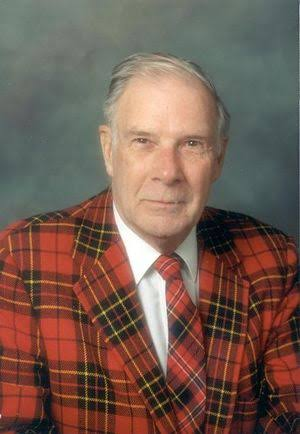
\includegraphics[width=1.80cm,height=2.20cm,keepaspectratio]{images/richardhamming.jpg}
      };
      \node[inner sep=0pt] at (1.50,0) {
        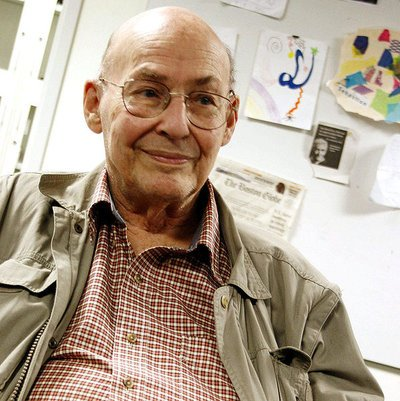
\includegraphics[width=1.80cm,height=2.20cm,keepaspectratio]{images/marvinminsky.jpg}
      };
      \node[inner sep=0pt] at (3.00,0) {
        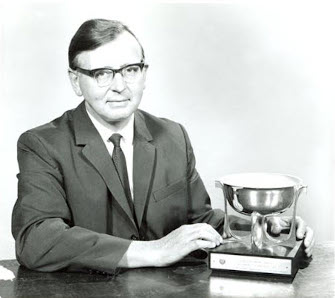
\includegraphics[width=1.80cm,height=2.20cm,keepaspectratio]{images/jameshwilkinson.jpg}
      };
  \end{tikzpicture}}
\end{frame}


\def\framesubject{AI 奠基人·结构化编程、Dijkstra·CODASYL 网状数据库模·《计算机程序设计艺术》、算法·人工智能、认知科学}
\begin{frame}{1971–1975}
\vspace{-2pt}
\centering
\scriptsize
\begin{tabular}{@{}
  >{\raggedright}m{2.5cm}
  >{\centering}m{1.0cm}
  >{\centering}m{1.95cm}
  >{\raggedleft}m{1.5cm}
  >{\raggedright}m{2.2cm}
  >{\raggedright\arraybackslash}m{2.35cm}
@{}}
\toprule
\rowcolor{turingbg}
\textbf{姓名} & \textbf{获奖年份} & \textbf{生卒} & \textbf{国籍} & \textbf{机构} & \textbf{研究领域} \\
\midrule
  \lrow{John McCarthy\kyotobadge\nsmbadge\cn{约翰·麦卡锡}}{1971}{1927–2011(享年84)}{美国}{Stanford University}{AI 奠基人，提出「人工智能」一词，Lisp 之父。}
  \lrow{Edsger W. Dijkstra\cn{埃德加·迪杰斯特拉}}{1972}{1930–2002(享年72)}{荷兰}{Eindhoven University of Technology}{结构化编程、Dijkstra 最短路径算法、并发原语。}
  \lrow{Charles Bachman\cn{查尔斯·巴赫曼}}{1973}{1924–2017(享年93)}{美国}{—}{CODASYL 网状数据库模型，数据库系统奠基人。}
  \lrow{Donald Knuth\kyotobadge\nsmbadge\cn{唐纳德·高德纳}}{1974}{1938–}{美国}{Stanford University}{《计算机程序设计艺术》、算法分析、TeX 排版系统。}
  \lrow{Allen Newell\cn{艾伦·纽厄尔}}{1975}{1927–1992(享年65)}{美国}{Carnegie Mellon University}{人工智能、认知科学，逻辑理论机。}
\bottomrule
\end{tabular}
\vspace{6pt}
  {\centering
  \begin{tikzpicture}
      \node[inner sep=0pt] at (-3.00,0) {
        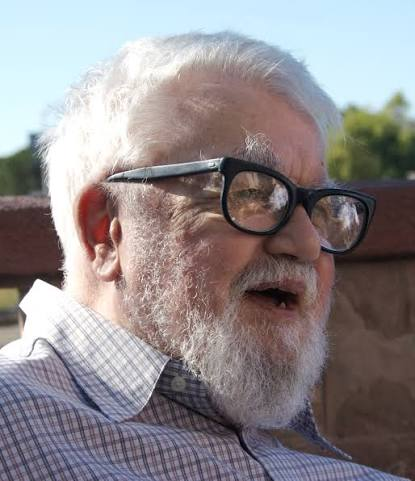
\includegraphics[width=1.80cm,height=2.20cm,keepaspectratio]{images/johnmccarthy.jpg}
      };
      \node[inner sep=0pt] at (-1.50,0) {
        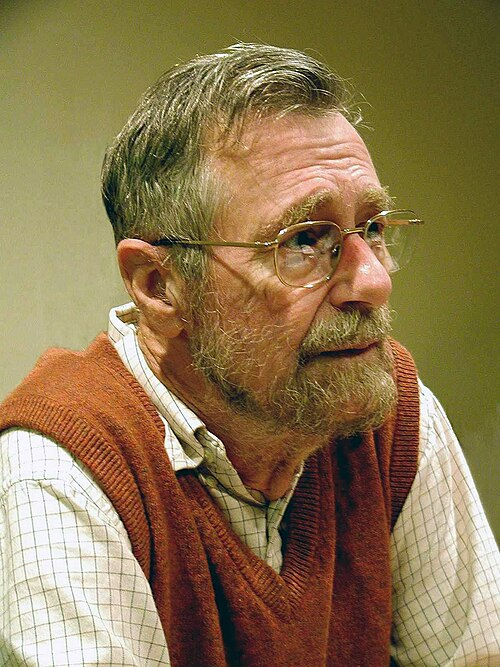
\includegraphics[width=1.80cm,height=2.20cm,keepaspectratio]{images/edsgerwdijkstra.jpg}
      };
      \node[inner sep=0pt] at (0.00,0) {
        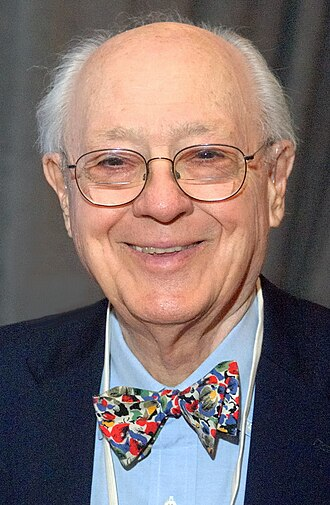
\includegraphics[width=1.80cm,height=2.20cm,keepaspectratio]{images/charlesbachman.jpg}
      };
      \node[inner sep=0pt] at (1.50,0) {
        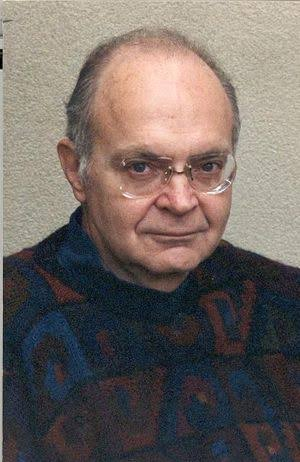
\includegraphics[width=1.80cm,height=2.20cm,keepaspectratio]{images/donaldknuth.jpg}
      };
      \node[inner sep=0pt] at (3.00,0) {
        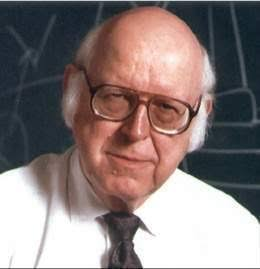
\includegraphics[width=1.80cm,height=2.20cm,keepaspectratio]{images/allennewell.jpg}
      };
  \end{tikzpicture}}
\end{frame}


\def\framesubject{认知科学·域理论·非确定性自动机、随机算法、米·Fortran 语言之父·程序设计方法学、Floyd }
\begin{frame}{1975–1978}
\vspace{-2pt}
\centering
\scriptsize
\begin{tabular}{@{}
  >{\raggedright}m{2.5cm}
  >{\centering}m{1.0cm}
  >{\centering}m{1.95cm}
  >{\raggedleft}m{1.5cm}
  >{\raggedright}m{2.2cm}
  >{\raggedright\arraybackslash}m{2.35cm}
@{}}
\toprule
\rowcolor{turingbg}
\textbf{姓名} & \textbf{获奖年份} & \textbf{生卒} & \textbf{国籍} & \textbf{机构} & \textbf{研究领域} \\
\midrule
  \lrow{Herbert A. Simon\nobelbadge\nsmbadge\cn{赫伯特·西蒙}}{1975}{1916–2001(享年85)}{美国}{Carnegie Mellon University}{认知科学，另获诺贝尔经济学奖（1978）——图灵+诺奖双料。}
  \lrow{Dana Scott\cn{达纳·斯科特}}{1976}{1932–}{美国}{Carnegie Mellon University}{域理论，为程序语义学奠定数学基础。}
  \lrow{Michael O. Rabin\cn{迈克尔·拉宾}}{1976}{1931–}{以色列/美国}{Harvard University}{非确定性自动机、随机算法、米勒-拉宾素性检验。}
  \lrow{John Backus\nsmbadge\cn{约翰·巴克斯}}{1977}{1924–2007(享年83)}{美国}{IBM}{Fortran 语言之父，BNF 文法描述编程语言语法。}
  \lrow{Robert W. Floyd\cn{罗伯特·弗洛伊德}}{1978}{1936–2001(享年65)}{美国}{Stanford University}{程序设计方法学、Floyd 算法（判圈/最短路径）。}
\bottomrule
\end{tabular}
\vspace{6pt}
  {\centering
  \begin{tikzpicture}
      \node[inner sep=0pt] at (-3.00,0) {
        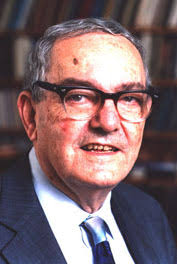
\includegraphics[width=1.80cm,height=2.20cm,keepaspectratio]{images/herbertasimon.jpg}
      };
      \node[inner sep=0pt] at (-1.50,0) {
        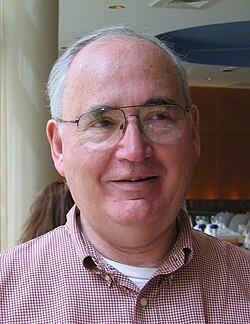
\includegraphics[width=1.80cm,height=2.20cm,keepaspectratio]{images/danascott.jpg}
      };
      \node[inner sep=0pt] at (0.00,0) {
        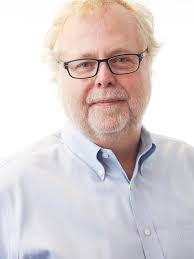
\includegraphics[width=1.80cm,height=2.20cm,keepaspectratio]{images/michaelorabin.jpg}
      };
      \node[inner sep=0pt] at (1.50,0) {
        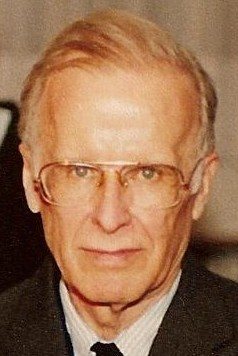
\includegraphics[width=1.80cm,height=2.20cm,keepaspectratio]{images/johnbackus.jpg}
      };
      \node[inner sep=0pt] at (3.00,0) {
        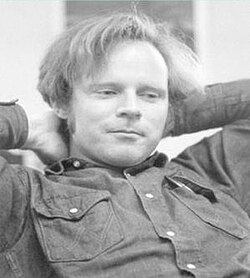
\includegraphics[width=1.80cm,height=2.20cm,keepaspectratio]{images/robertwfloyd.jpg}
      };
  \end{tikzpicture}}
\end{frame}


\def\framesubject{APL 语言·快速排序、Hoare 逻辑（·关系数据库模型·P 与 NP 问题、Cook·C 语言设计者、Unix 共}
\begin{frame}{1979–1983}
\vspace{-2pt}
\centering
\scriptsize
\begin{tabular}{@{}
  >{\raggedright}m{2.5cm}
  >{\centering}m{1.0cm}
  >{\centering}m{1.95cm}
  >{\raggedleft}m{1.5cm}
  >{\raggedright}m{2.2cm}
  >{\raggedright\arraybackslash}m{2.35cm}
@{}}
\toprule
\rowcolor{turingbg}
\textbf{姓名} & \textbf{获奖年份} & \textbf{生卒} & \textbf{国籍} & \textbf{机构} & \textbf{研究领域} \\
\midrule
  \lrow{Kenneth E. Iverson\cn{肯尼思·艾弗森}}{1979}{1920–2004(享年84)}{加拿大}{IBM}{APL 语言，交互式数组编程。}
  \lrow{Tony Hoare\kyotobadge\neumannbadge\cn{托尼·霍尔}}{1980}{1934–}{英国}{University of Oxford}{快速排序、Hoare 逻辑（程序验证）、CSP 通信顺序进程。}
  \lrow{Edgar F. Codd\cn{埃德加·科德}}{1981}{1923–2003(享年80)}{英国/美国}{IBM}{关系数据库模型，SQL 的理论根基。}
  \lrow{Stephen Cook\cn{史蒂芬·库克}}{1982}{1939–}{美国/加拿大}{University of Toronto}{P 与 NP 问题、Cook-Levin 定理，计算复杂性理论奠基人之一。}
  \lrow{Dennis Ritchie\japanbadge\ntmbadge\cn{丹尼斯·里奇}}{1983}{1941–2011(享年70)}{美国}{Bell Labs}{C 语言设计者、Unix 共同作者。}
\bottomrule
\end{tabular}
\vspace{6pt}
  {\centering
  \begin{tikzpicture}
      \node[inner sep=0pt] at (-3.00,0) {
        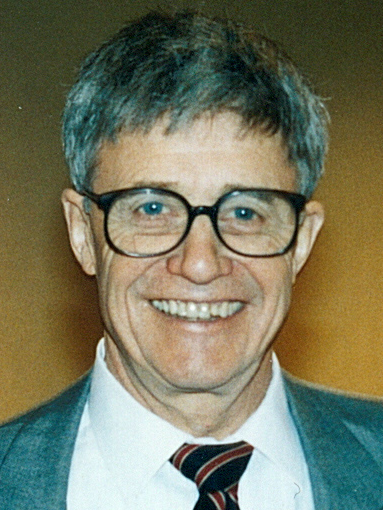
\includegraphics[width=1.80cm,height=2.20cm,keepaspectratio]{images/kennetheiverson.jpg}
      };
      \node[inner sep=0pt] at (-1.50,0) {
        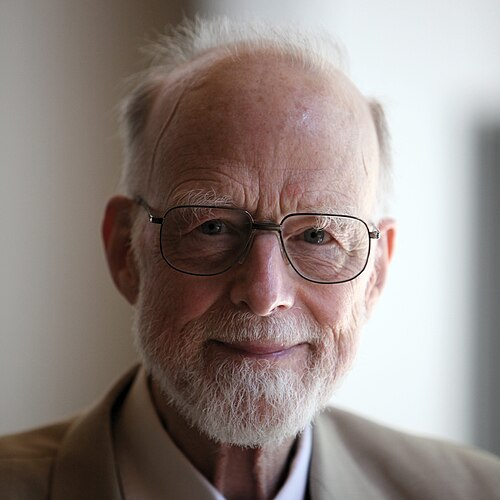
\includegraphics[width=1.80cm,height=2.20cm,keepaspectratio]{images/tonyhoare.jpg}
      };
      \node[inner sep=0pt] at (0.00,0) {
        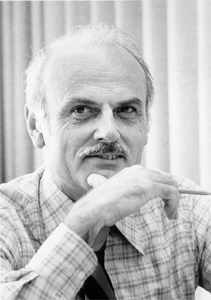
\includegraphics[width=1.80cm,height=2.20cm,keepaspectratio]{images/edgarfcodd.jpg}
      };
      \node[inner sep=0pt] at (1.50,0) {
        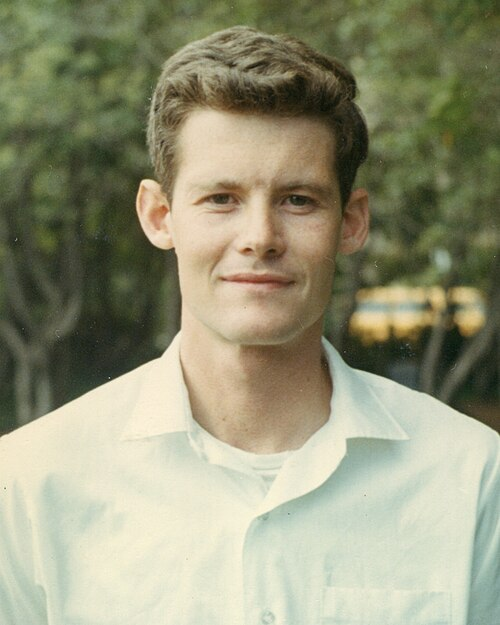
\includegraphics[width=1.80cm,height=2.20cm,keepaspectratio]{images/stephencook.jpg}
      };
      \node[inner sep=0pt] at (3.00,0) {
        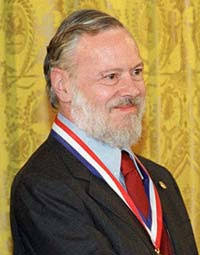
\includegraphics[width=1.80cm,height=2.20cm,keepaspectratio]{images/dennisritchie.jpg}
      };
  \end{tikzpicture}}
\end{frame}


\def\framesubject{Unix 操作系统与 C 语·Pascal、Modula ·NP 完全性理论、Karp ·算法设计与自动机理论·并查集、最近公共祖先、强连通}
\begin{frame}{1983–1986}
\vspace{-2pt}
\centering
\scriptsize
\begin{tabular}{@{}
  >{\raggedright}m{2.5cm}
  >{\centering}m{1.0cm}
  >{\centering}m{1.95cm}
  >{\raggedleft}m{1.5cm}
  >{\raggedright}m{2.2cm}
  >{\raggedright\arraybackslash}m{2.35cm}
@{}}
\toprule
\rowcolor{turingbg}
\textbf{姓名} & \textbf{获奖年份} & \textbf{生卒} & \textbf{国籍} & \textbf{机构} & \textbf{研究领域} \\
\midrule
  \lrow{Ken Thompson\japanbadge\ntmbadge\cn{肯·汤普森}}{1983}{1943–}{美国}{Bell Labs}{Unix 操作系统与 C 语言共同之父。}
  \lrow{Niklaus Wirth\cn{尼克劳斯·沃斯}}{1984}{1934–}{瑞士}{ETH Zurich}{Pascal、Modula 语言，结构化程序设计。}
  \lrow{Richard Karp\kyotobadge\eatcsbadge\nsmbadge\cn{理查德·卡普}}{1985}{1935–}{美国}{UC Berkeley}{NP 完全性理论、Karp 归约，组合优化的算法大师。}
  \lrow{John Hopcroft\cn{约翰·霍普克罗夫特}}{1986}{1939–}{美国}{Cornell University}{算法设计与自动机理论，图算法经典教材作者。}
  \lrow{Robert Tarjan\cn{罗伯特·塔扬}}{1986}{1948–}{美国}{Princeton University}{并查集、最近公共祖先、强连通分量等图算法的发明者。}
\bottomrule
\end{tabular}
\vspace{6pt}
  {\centering
  \begin{tikzpicture}
      \node[inner sep=0pt] at (-3.00,0) {
        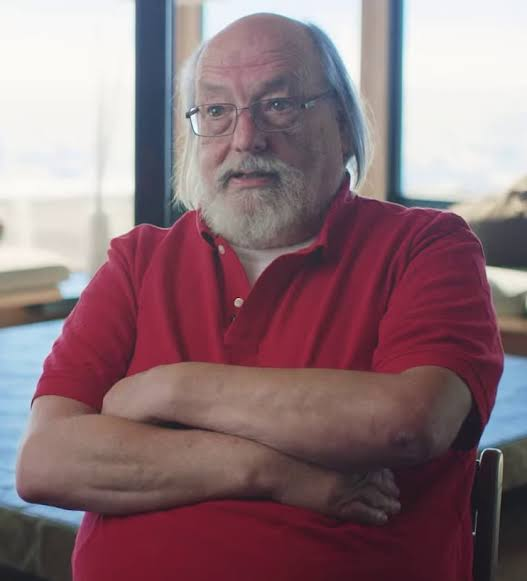
\includegraphics[width=1.80cm,height=2.20cm,keepaspectratio]{images/kenthompson.jpg}
      };
      \node[inner sep=0pt] at (-1.50,0) {
        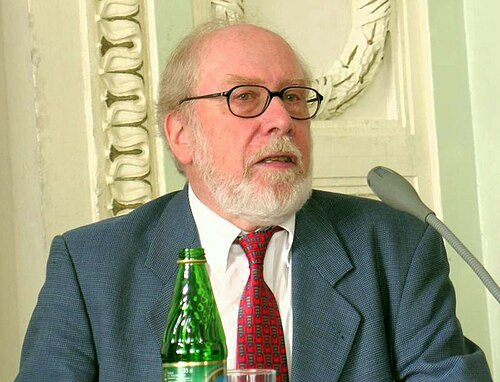
\includegraphics[width=1.80cm,height=2.20cm,keepaspectratio]{images/niklauswirth.jpg}
      };
      \node[inner sep=0pt] at (0.00,0) {
        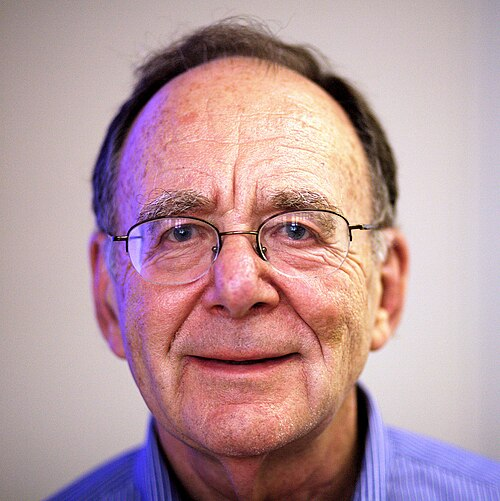
\includegraphics[width=1.80cm,height=2.20cm,keepaspectratio]{images/richardkarp.jpg}
      };
      \node[inner sep=0pt] at (1.50,0) {
        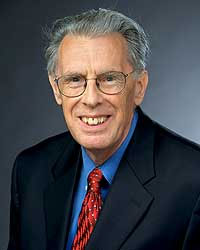
\includegraphics[width=1.80cm,height=2.20cm,keepaspectratio]{images/johnhopcroft.jpg}
      };
      \node[inner sep=0pt] at (3.00,0) {
        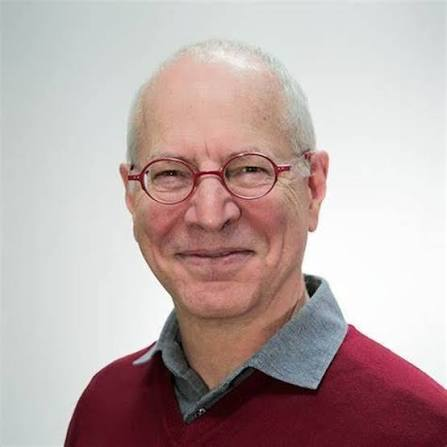
\includegraphics[width=1.80cm,height=2.20cm,keepaspectratio]{images/roberttarjan.jpg}
      };
  \end{tikzpicture}}
\end{frame}


\def\framesubject{RISC 架构、编译器优化·Sketchpad 交互式图·IEEE 754 浮点标准·分时系统 CTSS、Mult·ML 语言、LCF 定理证明}
\begin{frame}{1987–1991}
\vspace{-2pt}
\centering
\scriptsize
\begin{tabular}{@{}
  >{\raggedright}m{2.5cm}
  >{\centering}m{1.0cm}
  >{\centering}m{1.95cm}
  >{\raggedleft}m{1.5cm}
  >{\raggedright}m{2.2cm}
  >{\raggedright\arraybackslash}m{2.35cm}
@{}}
\toprule
\rowcolor{turingbg}
\textbf{姓名} & \textbf{获奖年份} & \textbf{生卒} & \textbf{国籍} & \textbf{机构} & \textbf{研究领域} \\
\midrule
  \lrow{John Cocke\cn{约翰·科克}}{1987}{1925–2002(享年77)}{美国}{IBM}{RISC 架构、编译器优化，IBM 体系结构先驱。}
  \lrow{Ivan Sutherland\kyotobadge\neumannbadge\cn{伊万·萨瑟兰}}{1988}{1938–}{美国}{—}{Sketchpad 交互式图形系统，计算机图形学之父。}
  \lrow{William Kahan\nsmbadge\cn{威廉·卡汉}}{1989}{1933–}{加拿大/美国}{UC Berkeley}{IEEE 754 浮点标准，数值分析大师。}
  \lrow{Fernando J. Corbató\cn{费尔南多·科巴托}}{1990}{1926–2019(享年93)}{美国}{MIT}{分时系统 CTSS、Multics，操作系统奠基人。}
  \lrow{Robin Milner\cn{罗宾·米尔纳}}{1991}{1934–2010(享年76)}{英国}{University of Edinburgh}{ML 语言、LCF 定理证明、$\pi$ 演算（并发理论）。}
\bottomrule
\end{tabular}
\vspace{6pt}
  {\centering
  \begin{tikzpicture}
      \node[inner sep=0pt] at (-3.00,0) {
        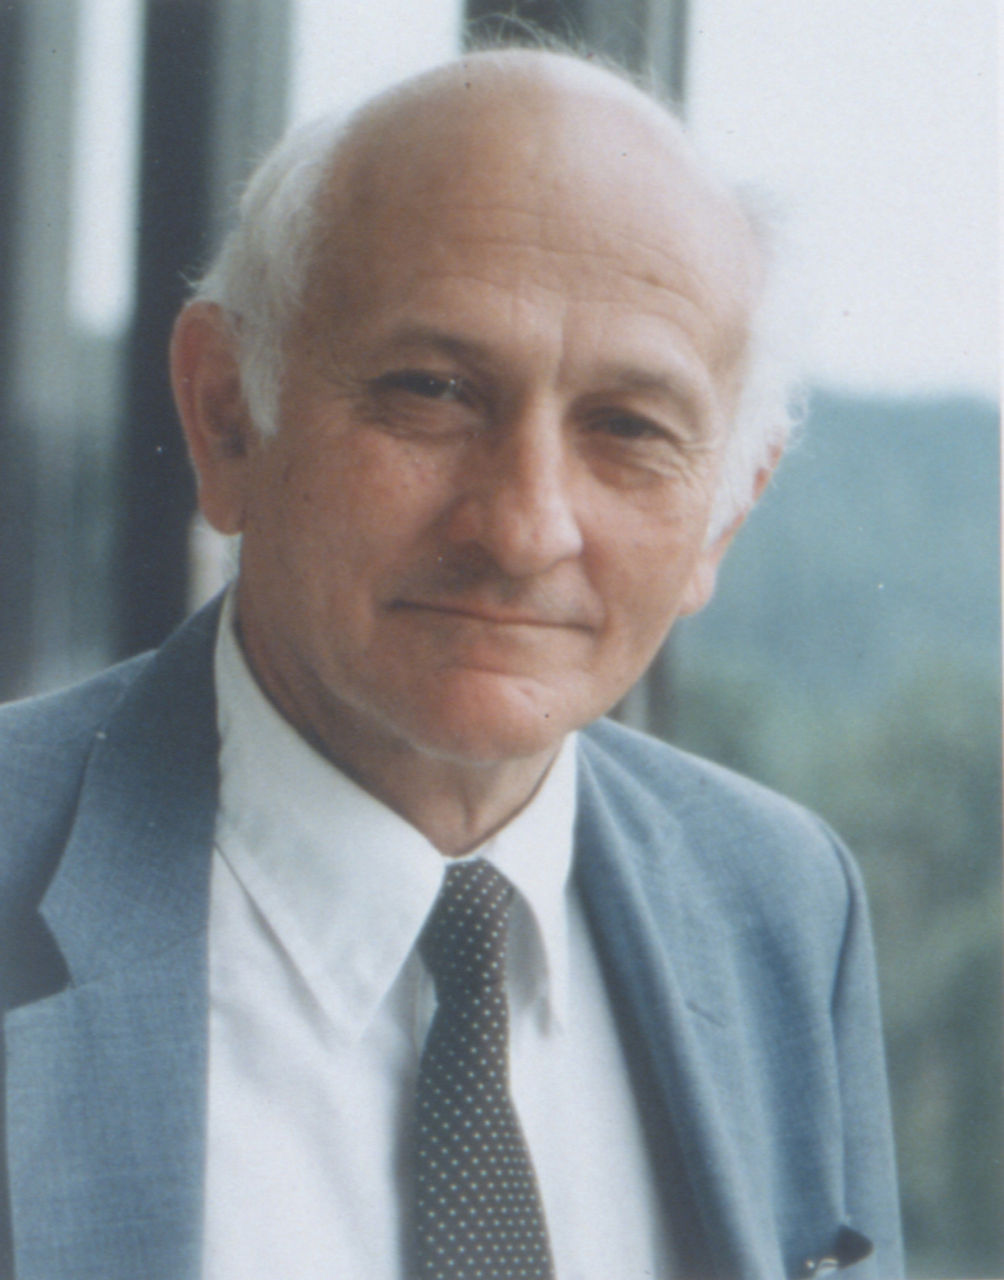
\includegraphics[width=1.80cm,height=2.20cm,keepaspectratio]{images/johncocke.jpg}
      };
      \node[inner sep=0pt] at (-1.50,0) {
        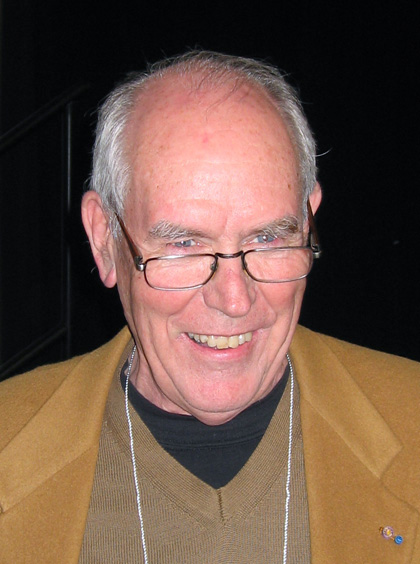
\includegraphics[width=1.80cm,height=2.20cm,keepaspectratio]{images/ivansutherland.jpg}
      };
      \node[inner sep=0pt] at (0.00,0) {
        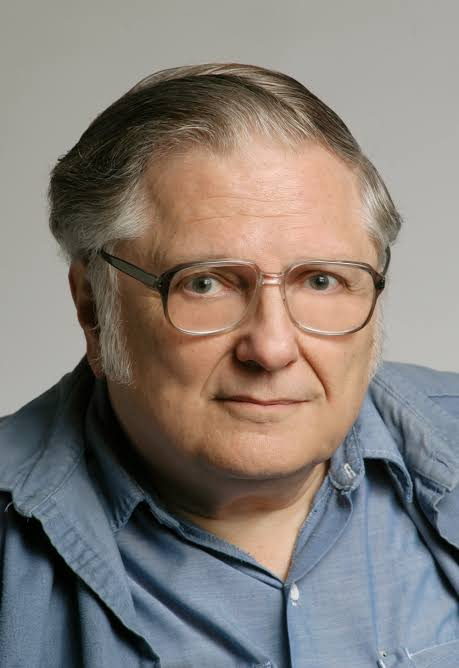
\includegraphics[width=1.80cm,height=2.20cm,keepaspectratio]{images/williamkahan.jpg}
      };
      \node[inner sep=0pt] at (1.50,0) {
        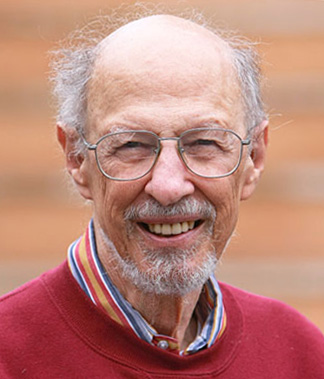
\includegraphics[width=1.80cm,height=2.20cm,keepaspectratio]{images/fernandojcorbato.jpg}
      };
      \node[inner sep=0pt] at (3.00,0) {
        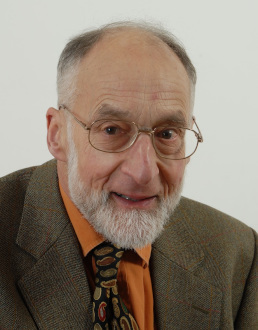
\includegraphics[width=1.80cm,height=2.20cm,keepaspectratio]{images/robinmilner.jpg}
      };
  \end{tikzpicture}}
\end{frame}


\def\framesubject{分布式系统、安全与容错·计算复杂性分层定理·计算复杂性理论奠基·专家系统、知识工程·人工智能、语音识别。}
\begin{frame}{1992–1994}
\vspace{-2pt}
\centering
\scriptsize
\begin{tabular}{@{}
  >{\raggedright}m{2.5cm}
  >{\centering}m{1.0cm}
  >{\centering}m{1.95cm}
  >{\raggedleft}m{1.5cm}
  >{\raggedright}m{2.2cm}
  >{\raggedright\arraybackslash}m{2.35cm}
@{}}
\toprule
\rowcolor{turingbg}
\textbf{姓名} & \textbf{获奖年份} & \textbf{生卒} & \textbf{国籍} & \textbf{机构} & \textbf{研究领域} \\
\midrule
  \lrow{Butler W. Lampson\cn{巴特勒·兰普森}}{1992}{1943–}{美国}{Microsoft Research}{分布式系统、安全与容错，个人计算愿景。}
  \lrow{Juris Hartmanis\cn{尤里斯·哈特马尼斯}}{1993}{1928–2022(享年94)}{美国/拉脱维亚}{Cornell University}{计算复杂性分层定理，复杂性理论共同奠基人。}
  \lrow{Richard E. Stearns\cn{理查德·斯特恩斯}}{1993}{1936–}{美国}{SUNY Albany}{计算复杂性理论奠基，与 Hartmanis 同获 1993 年奖。}
  \lrow{Edward Feigenbaum\cn{爱德华·费根鲍姆}}{1994}{1936–}{美国}{Stanford University}{专家系统、知识工程，AI 应用先驱。}
  \lrow{Raj Reddy\cn{拉吉·雷迪}}{1994}{1937–}{美国/印度}{Carnegie Mellon University}{人工智能、语音识别。}
\bottomrule
\end{tabular}
\vspace{6pt}
  {\centering
  \begin{tikzpicture}
      \node[inner sep=0pt] at (-3.00,0) {
        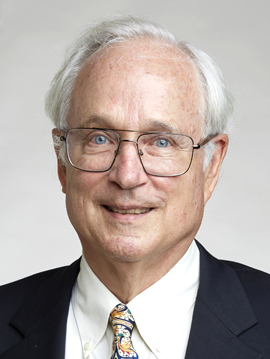
\includegraphics[width=1.80cm,height=2.20cm,keepaspectratio]{images/butlerwlampson.jpg}
      };
      \node[inner sep=0pt] at (-1.50,0) {
        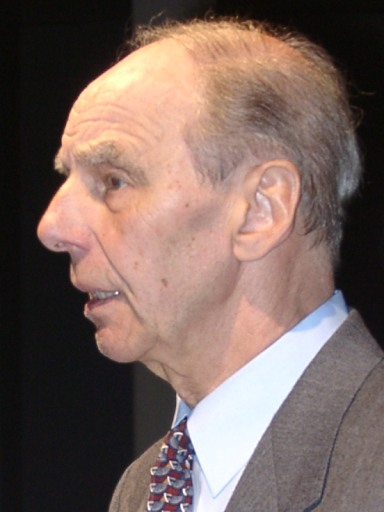
\includegraphics[width=1.80cm,height=2.20cm,keepaspectratio]{images/jurishartmanis.jpg}
      };
      \node[inner sep=0pt] at (0.00,0) {
        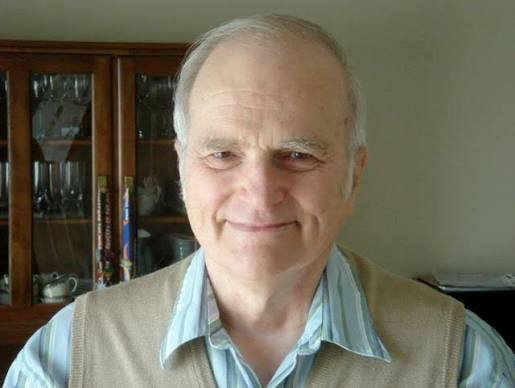
\includegraphics[width=1.80cm,height=2.20cm,keepaspectratio]{images/richardestearns.jpg}
      };
      \node[inner sep=0pt] at (1.50,0) {
        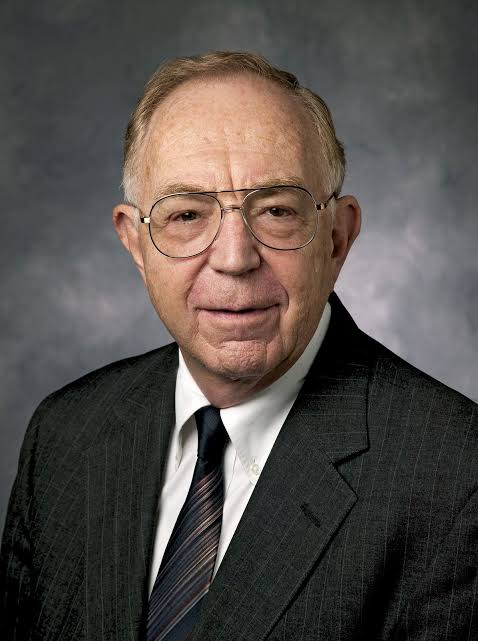
\includegraphics[width=1.80cm,height=2.20cm,keepaspectratio]{images/edwardfeigenbaum.jpg}
      };
      \node[inner sep=0pt] at (3.00,0) {
        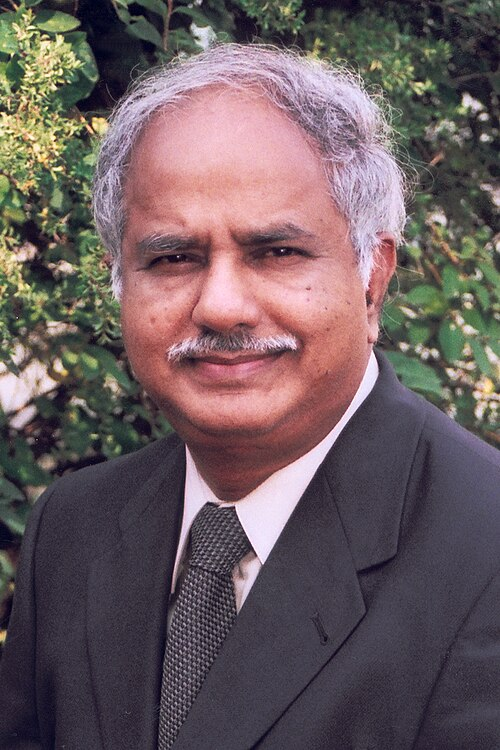
\includegraphics[width=1.80cm,height=2.20cm,keepaspectratio]{images/rajreddy.jpg}
      };
  \end{tikzpicture}}
\end{frame}


\def\framesubject{计算复杂性、Blum Blu·时态逻辑、程序验证·鼠标发明者、超文本、图形交互·事务处理、数据库系统与在线分·OS/360 软件工程、《人}
\begin{frame}{1995–1999}
\vspace{-2pt}
\centering
\scriptsize
\begin{tabular}{@{}
  >{\raggedright}m{2.5cm}
  >{\centering}m{1.0cm}
  >{\centering}m{1.95cm}
  >{\raggedleft}m{1.5cm}
  >{\raggedright}m{2.2cm}
  >{\raggedright\arraybackslash}m{2.35cm}
@{}}
\toprule
\rowcolor{turingbg}
\textbf{姓名} & \textbf{获奖年份} & \textbf{生卒} & \textbf{国籍} & \textbf{机构} & \textbf{研究领域} \\
\midrule
  \lrow{Manuel Blum\cn{曼努埃尔·布鲁姆}}{1995}{1938–}{美国}{Carnegie Mellon University}{计算复杂性、Blum Blum Shub 伪随机生成器。}
  \lrow{Amir Pnueli\cn{阿米尔·普努利}}{1996}{1941–2009(享年68)}{以色列}{Weizmann Institute}{时态逻辑、程序验证，反应系统形式化。}
  \lrow{Douglas Engelbart\cn{道格拉斯·恩格尔巴特}}{1997}{1925–2013(享年88)}{美国}{—}{鼠标发明者、超文本、图形交互（NLS）。}
  \lrow{Jim Gray\cn{吉姆·格雷}}{1998}{1944–2012(享年68)}{美国}{Microsoft Research}{事务处理、数据库系统与在线分析处理。}
  \lrow{Fred Brooks\cn{弗雷德·布鲁克斯}}{1999}{1931–2022(享年91)}{美国}{University of North Carolina}{OS/360 软件工程、《人月神话》作者。}
\bottomrule
\end{tabular}
\vspace{6pt}
  {\centering
  \begin{tikzpicture}
      \node[inner sep=0pt] at (-3.00,0) {
        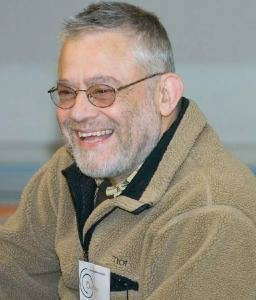
\includegraphics[width=1.80cm,height=2.20cm,keepaspectratio]{images/manuelblum.jpg}
      };
      \node[inner sep=0pt] at (-1.50,0) {
        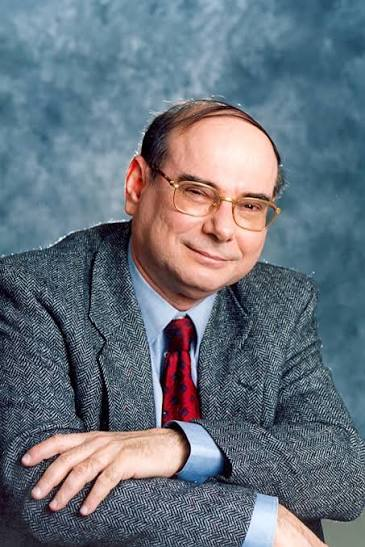
\includegraphics[width=1.80cm,height=2.20cm,keepaspectratio]{images/amirpnueli.jpg}
      };
      \node[inner sep=0pt] at (0.00,0) {
        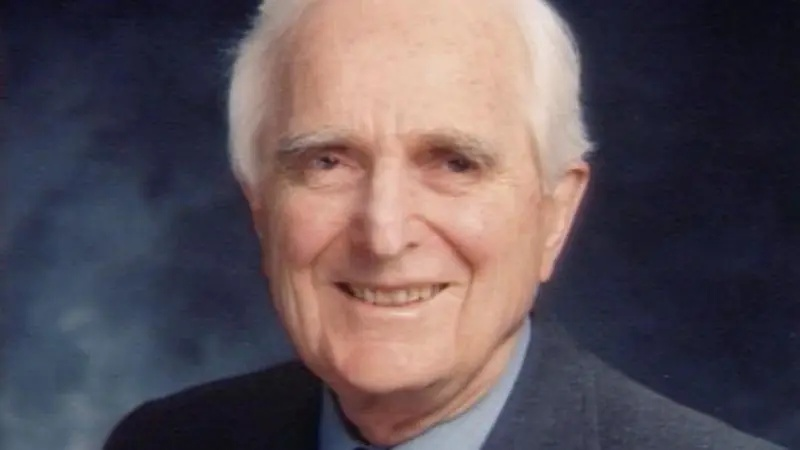
\includegraphics[width=1.80cm,height=2.20cm,keepaspectratio]{images/douglasengelbart.jpg}
      };
      \node[inner sep=0pt] at (1.50,0) {
        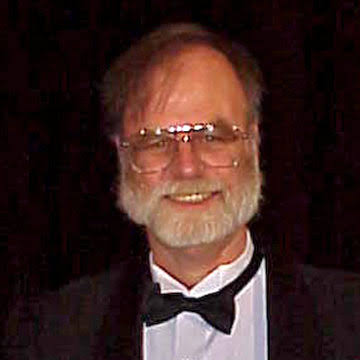
\includegraphics[width=1.80cm,height=2.20cm,keepaspectratio]{images/jimgray.jpg}
      };
      \node[inner sep=0pt] at (3.00,0) {
        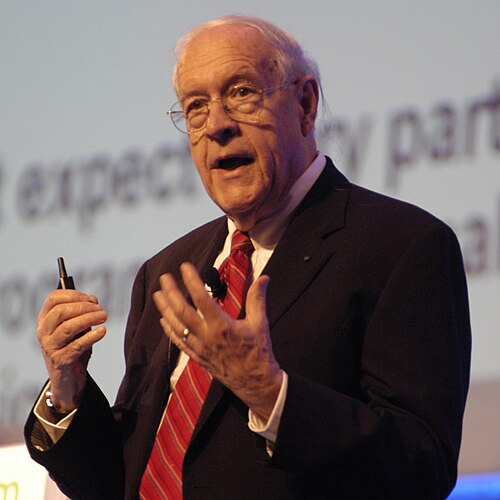
\includegraphics[width=1.80cm,height=2.20cm,keepaspectratio]{images/fredbrooks.jpg}
      };
  \end{tikzpicture}}
\end{frame}


\def\framesubject{通信复杂性、密码学、量子计算·面向对象编程（Simula ·面向对象编程（Simula ·RSA 三杰之一·RSA 三杰之一}
\begin{frame}{2000–2002}
\vspace{-2pt}
\centering
\scriptsize
\begin{tabular}{@{}
  >{\raggedright}m{2.5cm}
  >{\centering}m{1.0cm}
  >{\centering}m{1.95cm}
  >{\raggedleft}m{1.5cm}
  >{\raggedright}m{2.2cm}
  >{\raggedright\arraybackslash}m{2.35cm}
@{}}
\toprule
\rowcolor{turingbg}
\textbf{姓名} & \textbf{获奖年份} & \textbf{生卒} & \textbf{国籍} & \textbf{机构} & \textbf{研究领域} \\
\midrule
  \lrow{Andrew Yao\kyotobadge\cn{姚期智}}{2000}{1946–}{美国/中国}{Princeton University / Tsinghua}{通信复杂性、密码学、量子计算——首位华人图灵奖得主。}
  \lrow{Kristen Nygaard\cn{克里斯汀·尼加德}}{2001}{1926–2002(享年76)}{挪威}{University of Oslo}{面向对象编程（Simula 语言），与 Dahl 同获 2001 年奖。}
  \lrow{Ole-Johan Dahl\cn{奥利-约翰·达尔}}{2001}{1931–2002(享年71)}{挪威}{University of Oslo}{面向对象编程（Simula 语言），OOP 先驱。}
  \lrow{Adi Shamir\wolfbadge\frsbadge\cn{阿迪·沙米尔}}{2002}{1952–}{以色列}{Weizmann Institute}{RSA 三杰之一，Shamir 秘密共享、密码分析。}
  \lrow{Leonard Adleman\cn{伦纳德·阿德尔曼}}{2002}{1945–}{美国}{MIT}{RSA 三杰之一，DNA 计算先驱。}
\bottomrule
\end{tabular}
\vspace{6pt}
  {\centering
  \begin{tikzpicture}
      \node[inner sep=0pt] at (-3.00,0) {
        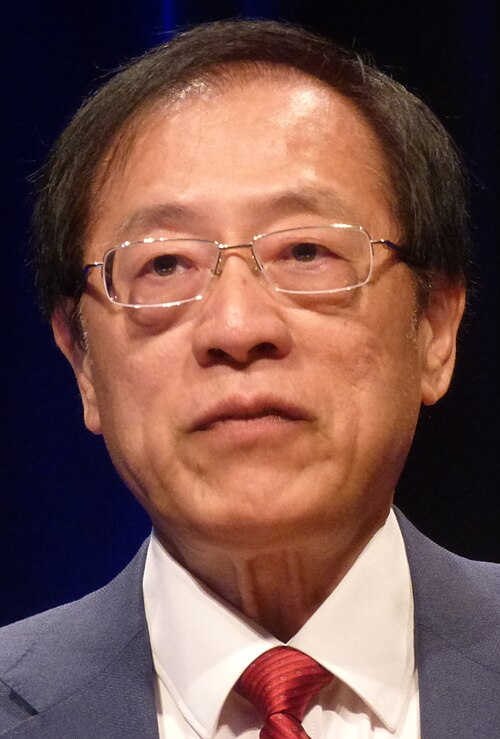
\includegraphics[width=1.80cm,height=2.20cm,keepaspectratio]{images/andrewyao.jpg}
      };
      \node[inner sep=0pt] at (-1.50,0) {
        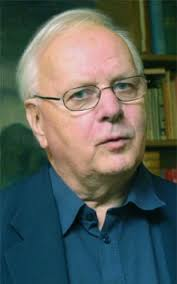
\includegraphics[width=1.80cm,height=2.20cm,keepaspectratio]{images/kristennygaard.jpg}
      };
      \node[inner sep=0pt] at (0.00,0) {
        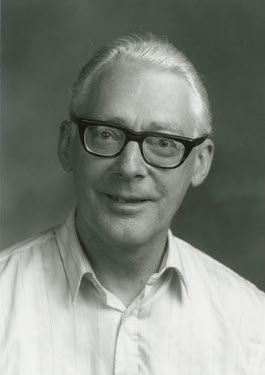
\includegraphics[width=1.80cm,height=2.20cm,keepaspectratio]{images/olejohandahl.jpg}
      };
      \node[inner sep=0pt] at (1.50,0) {
        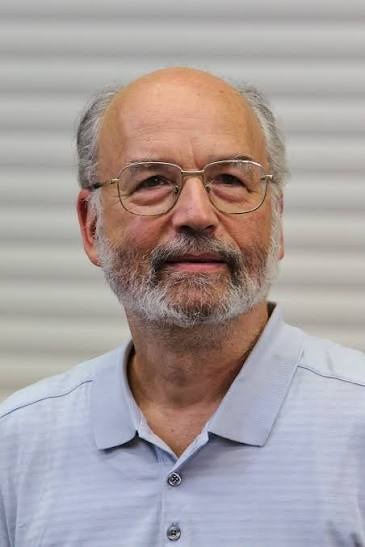
\includegraphics[width=1.80cm,height=2.20cm,keepaspectratio]{images/adishamir.jpg}
      };
      \node[inner sep=0pt] at (3.00,0) {
        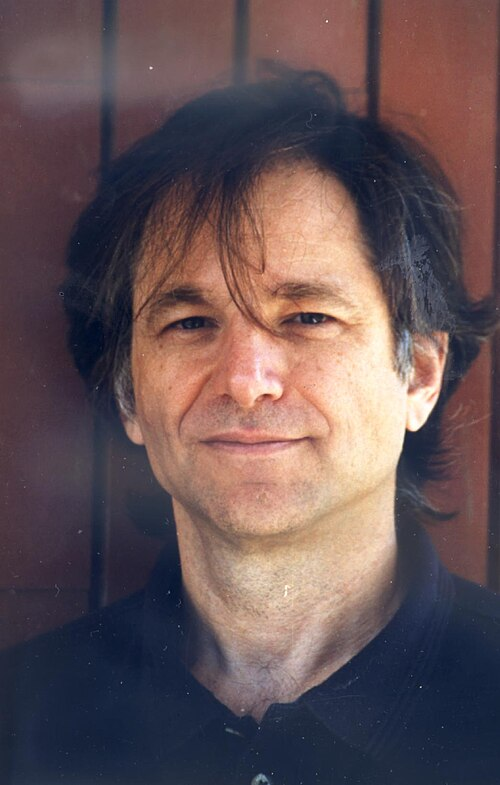
\includegraphics[width=1.80cm,height=2.20cm,keepaspectratio]{images/leonardadleman.jpg}
      };
  \end{tikzpicture}}
\end{frame}


\def\framesubject{RSA 公钥密码学三杰之一。·Smalltalk、面向对象·TCP/IP 协议共同设计者·TCP/IP 协议共同设计者·Algol 60、BNF 文}
\begin{frame}{2002–2005}
\vspace{-2pt}
\centering
\scriptsize
\begin{tabular}{@{}
  >{\raggedright}m{2.5cm}
  >{\centering}m{1.0cm}
  >{\centering}m{1.95cm}
  >{\raggedleft}m{1.5cm}
  >{\raggedright}m{2.2cm}
  >{\raggedright\arraybackslash}m{2.35cm}
@{}}
\toprule
\rowcolor{turingbg}
\textbf{姓名} & \textbf{获奖年份} & \textbf{生卒} & \textbf{国籍} & \textbf{机构} & \textbf{研究领域} \\
\midrule
  \lrow{Ronald Rivest\marconibadge\cn{罗纳德·里维斯特}}{2002}{1947–}{美国}{MIT}{RSA 公钥密码学三杰之一。}
  \lrow{Alan Kay\kyotobadge\cn{艾伦·凯}}{2003}{1940–}{美国}{—}{Smalltalk、面向对象思想、图形用户界面，个人计算愿景。}
  \lrow{Robert Kahn\cn{罗伯特·卡恩}}{2004}{1938–}{美国}{—}{TCP/IP 协议共同设计者，互联网架构奠基。}
  \lrow{Vint Cerf\japanbadge\marconibadge\ntmbadge\cn{文顿·瑟夫}}{2004}{1943–}{美国}{—}{TCP/IP 协议共同设计者，互联网之父之一。}
  \lrow{Peter Naur\cn{彼得·诺尔}}{2005}{1928–2016(享年88)}{丹麦}{—}{Algol 60、BNF 文法、软件工程方法论。}
\bottomrule
\end{tabular}
\vspace{6pt}
  {\centering
  \begin{tikzpicture}
      \node[inner sep=0pt] at (-3.00,0) {
        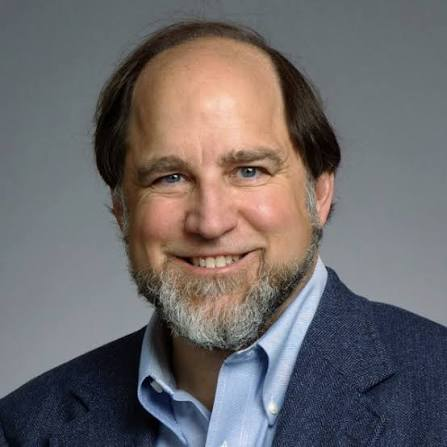
\includegraphics[width=1.80cm,height=2.20cm,keepaspectratio]{images/ronaldrivest.jpg}
      };
      \node[inner sep=0pt] at (-1.50,0) {
        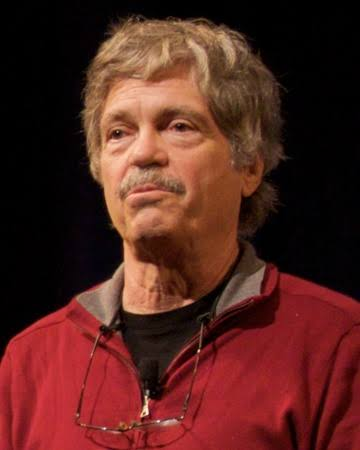
\includegraphics[width=1.80cm,height=2.20cm,keepaspectratio]{images/alankay.jpg}
      };
      \node[inner sep=0pt] at (0.00,0) {
        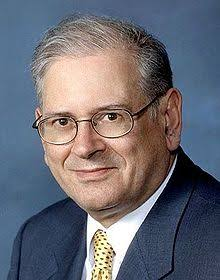
\includegraphics[width=1.80cm,height=2.20cm,keepaspectratio]{images/robertkahn.jpg}
      };
      \node[inner sep=0pt] at (1.50,0) {
        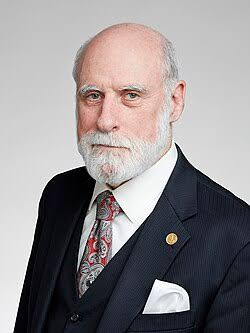
\includegraphics[width=1.80cm,height=2.20cm,keepaspectratio]{images/vintcerf.jpg}
      };
      \node[inner sep=0pt] at (3.00,0) {
        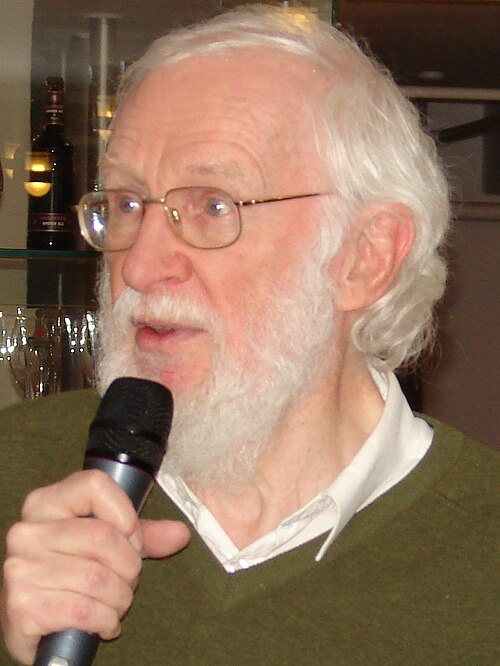
\includegraphics[width=1.80cm,height=2.20cm,keepaspectratio]{images/peternaur.jpg}
      };
  \end{tikzpicture}}
\end{frame}


\def\framesubject{编译器优化、并行计算·模型检验、时态逻辑。·模型检验（Model Che·模型检验、并发系统验证。·分布式系统、数据抽象、Lis}
\begin{frame}{2006–2008}
\vspace{-2pt}
\centering
\scriptsize
\begin{tabular}{@{}
  >{\raggedright}m{2.5cm}
  >{\centering}m{1.0cm}
  >{\centering}m{1.95cm}
  >{\raggedleft}m{1.5cm}
  >{\raggedright}m{2.2cm}
  >{\raggedright\arraybackslash}m{2.35cm}
@{}}
\toprule
\rowcolor{turingbg}
\textbf{姓名} & \textbf{获奖年份} & \textbf{生卒} & \textbf{国籍} & \textbf{机构} & \textbf{研究领域} \\
\midrule
  \lrow{Frances E. Allen\cn{弗朗西丝·艾伦}}{2006}{1932–2020(享年88)}{美国}{IBM}{编译器优化、并行计算，首位女性图灵奖得主。}
  \lrow{E. Allen Emerson\cn{艾伦·埃默森}}{2007}{1954–}{美国}{University of Texas at Austin}{模型检验、时态逻辑。}
  \lrow{Edmund M. Clarke\cn{埃德蒙·克拉克}}{2007}{1945–2020(享年75)}{美国}{Carnegie Mellon University}{模型检验（Model Checking）奠基人。}
  \lrow{Joseph Sifakis\cn{约瑟夫·西法基斯}}{2007}{1946–}{法国/希腊}{Verimag}{模型检验、并发系统验证。}
  \lrow{Barbara Liskov\neumannbadge\cn{芭芭拉·利斯科夫}}{2008}{1939–}{美国}{MIT}{分布式系统、数据抽象、Liskov 替换原则，第二位女性得主。}
\bottomrule
\end{tabular}
\vspace{6pt}
  {\centering
  \begin{tikzpicture}
      \node[inner sep=0pt] at (-3.00,0) {
        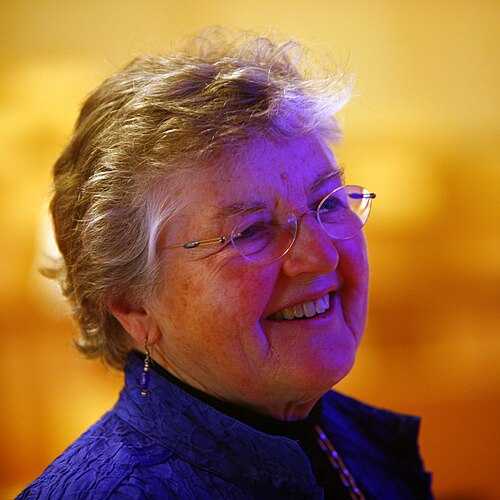
\includegraphics[width=1.80cm,height=2.20cm,keepaspectratio]{images/franceseallen.jpg}
      };
      \node[inner sep=0pt] at (-1.50,0) {
        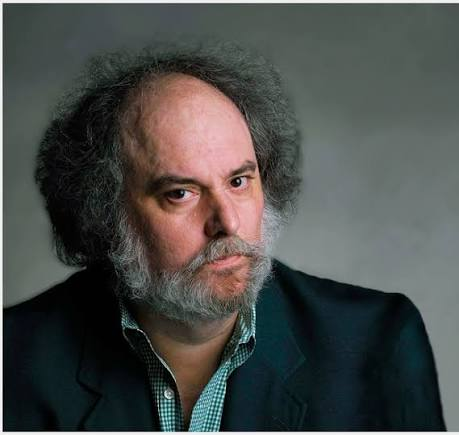
\includegraphics[width=1.80cm,height=2.20cm,keepaspectratio]{images/eallenemerson.jpg}
      };
      \node[inner sep=0pt] at (0.00,0) {
        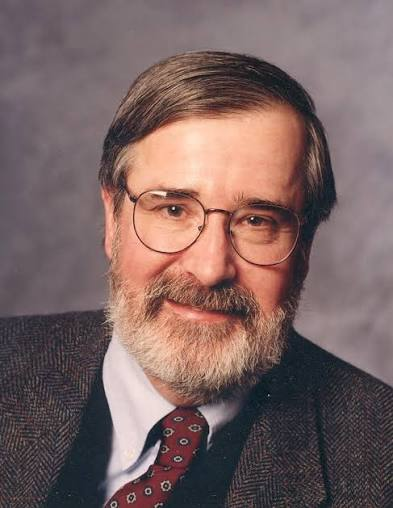
\includegraphics[width=1.80cm,height=2.20cm,keepaspectratio]{images/edmundmclarke.jpg}
      };
      \node[inner sep=0pt] at (1.50,0) {
        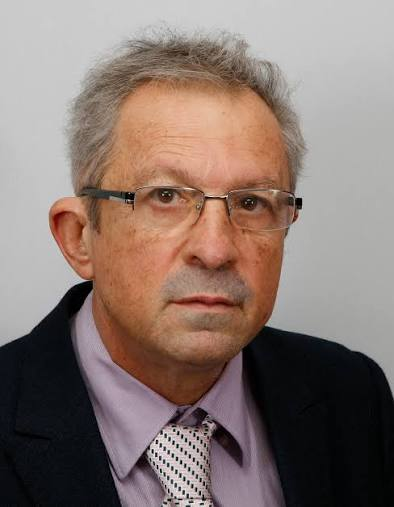
\includegraphics[width=1.80cm,height=2.20cm,keepaspectratio]{images/josephsifakis.jpg}
      };
      \node[inner sep=0pt] at (3.00,0) {
        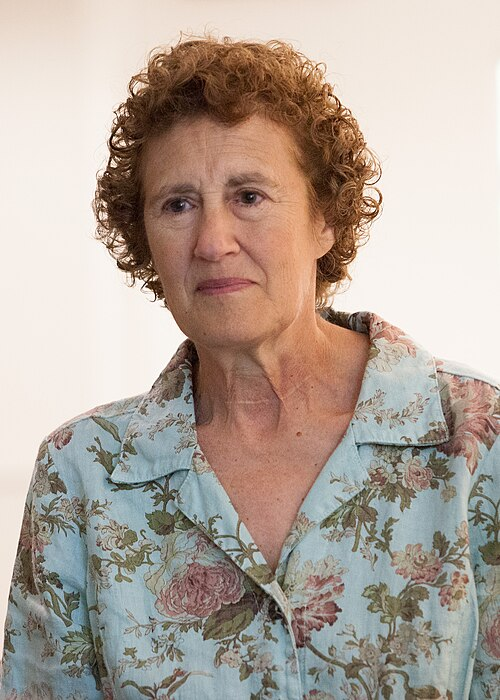
\includegraphics[width=1.80cm,height=2.20cm,keepaspectratio]{images/barbaraliskov.jpg}
      };
  \end{tikzpicture}}
\end{frame}


\def\framesubject{Alto 个人电脑、以太网、·PAC 学习理论、VLSI ·贝叶斯网络、因果推断·概率加密、零知识证明·零知识证明、可验证随机函数。}
\begin{frame}{2009–2012}
\vspace{-2pt}
\centering
\scriptsize
\begin{tabular}{@{}
  >{\raggedright}m{2.5cm}
  >{\centering}m{1.0cm}
  >{\centering}m{1.95cm}
  >{\raggedleft}m{1.5cm}
  >{\raggedright}m{2.2cm}
  >{\raggedright\arraybackslash}m{2.35cm}
@{}}
\toprule
\rowcolor{turingbg}
\textbf{姓名} & \textbf{获奖年份} & \textbf{生卒} & \textbf{国籍} & \textbf{机构} & \textbf{研究领域} \\
\midrule
  \lrow{Charles P. Thacker\cn{查尔斯·萨克}}{2009}{1943–2017(享年74)}{美国}{Microsoft Research}{Alto 个人电脑、以太网、平板显示。}
  \lrow{Leslie Valiant\nevanlinnabadge\eatcsbadge\cn{莱斯利·瓦利安特}}{2010}{1949–}{英国/美国}{Harvard University}{PAC 学习理论、VLSI 计算复杂度，学习理论奠基人。}
  \lrow{Judea Pearl\nsmbadge\rumelhartbadge\cn{朱迪亚·珀尔}}{2011}{1936–}{美国/以色列}{UCLA}{贝叶斯网络、因果推断，AI 概率推理奠基人。}
  \lrow{Shafi Goldwasser\godelbadge\nasbadge\cn{沙菲·戈德瓦瑟}}{2012}{1958–}{美国/以色列}{MIT / Weizmann}{概率加密、零知识证明，现代密码学奠基。}
  \lrow{Silvio Micali\godelbadge\nasbadge\cn{西尔维奥·米卡利}}{2012}{1954–}{意大利/美国}{MIT}{零知识证明、可验证随机函数。}
\bottomrule
\end{tabular}
\vspace{6pt}
  {\centering
  \begin{tikzpicture}
      \node[inner sep=0pt] at (-3.00,0) {
        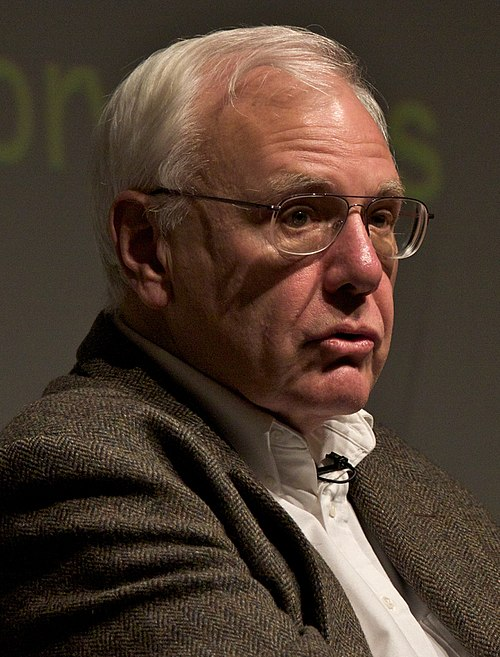
\includegraphics[width=1.80cm,height=2.20cm,keepaspectratio]{images/charlespthacker.jpg}
      };
      \node[inner sep=0pt] at (-1.50,0) {
        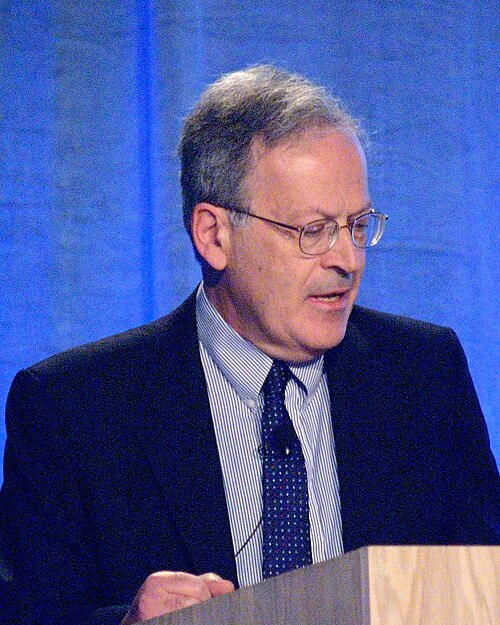
\includegraphics[width=1.80cm,height=2.20cm,keepaspectratio]{images/leslievaliant.jpg}
      };
      \node[inner sep=0pt] at (0.00,0) {
        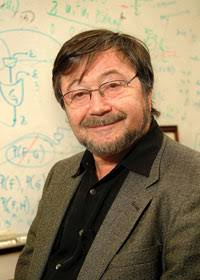
\includegraphics[width=1.80cm,height=2.20cm,keepaspectratio]{images/judeapearl.jpg}
      };
      \node[inner sep=0pt] at (1.50,0) {
        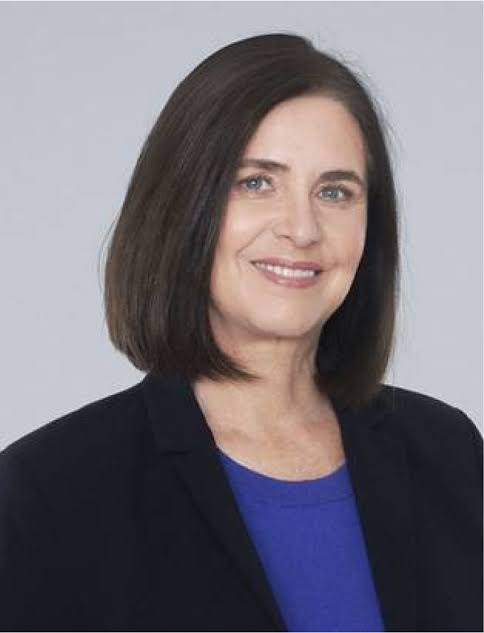
\includegraphics[width=1.80cm,height=2.20cm,keepaspectratio]{images/shafigoldwasser.jpg}
      };
      \node[inner sep=0pt] at (3.00,0) {
        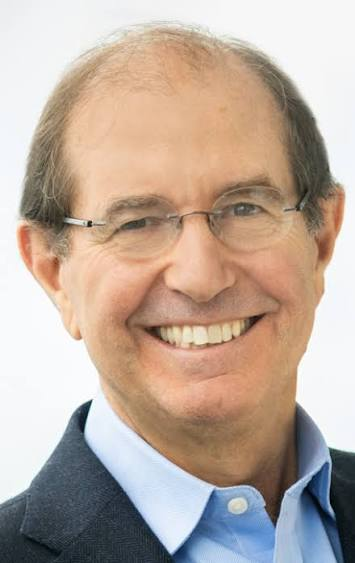
\includegraphics[width=1.80cm,height=2.20cm,keepaspectratio]{images/silviomicali.jpg}
      };
  \end{tikzpicture}}
\end{frame}


\def\framesubject{Paxos 共识算法、时序逻·Ingres、Postgre·公钥密码学（Diffie-H·公钥密码学（Diffie-H·万维网（WWW）发明者}
\begin{frame}{2013–2016}
\vspace{-2pt}
\centering
\scriptsize
\begin{tabular}{@{}
  >{\raggedright}m{2.5cm}
  >{\centering}m{1.0cm}
  >{\centering}m{1.95cm}
  >{\raggedleft}m{1.5cm}
  >{\raggedright}m{2.2cm}
  >{\raggedright\arraybackslash}m{2.35cm}
@{}}
\toprule
\rowcolor{turingbg}
\textbf{姓名} & \textbf{获奖年份} & \textbf{生卒} & \textbf{国籍} & \textbf{机构} & \textbf{研究领域} \\
\midrule
  \lrow{Leslie Lamport\neumannbadge\nasbadge\cn{莱斯利·兰波特}}{2013}{1941–}{美国}{Microsoft Research}{Paxos 共识算法、时序逻辑、LaTeX。}
  \lrow{Michael Stonebraker\cn{迈克尔·斯通布雷克}}{2014}{1943–}{美国}{MIT}{Ingres、PostgreSQL 数据库系统，流处理先驱。}
  \lrow{Martin Hellman\hammingbadge\marconibadge\cn{马丁·赫尔曼}}{2015}{1945–}{美国}{Stanford University}{公钥密码学（Diffie-Hellman 密钥交换）。}
  \lrow{Whitfield Diffie\hammingbadge\marconibadge\frsbadge\cn{惠特菲尔德·迪菲}}{2015}{1944–}{美国}{—}{公钥密码学（Diffie-Hellman 密钥交换）。}
  \lrow{Tim Berners-Lee\nasbadge\frsbadge\cn{蒂姆·伯纳斯-李}}{2016}{1955–}{英国}{W3C / MIT}{万维网（WWW）发明者，HTML、HTTP、URL。}
\bottomrule
\end{tabular}
\vspace{6pt}
  {\centering
  \begin{tikzpicture}
      \node[inner sep=0pt] at (-3.00,0) {
        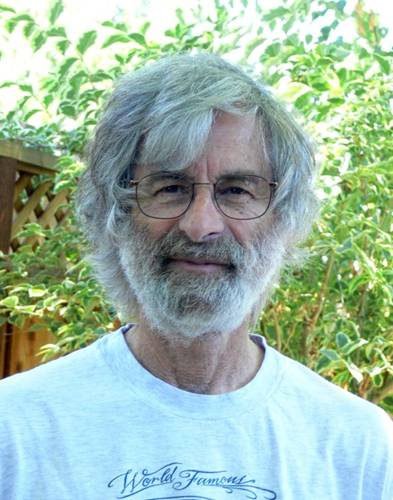
\includegraphics[width=1.80cm,height=2.20cm,keepaspectratio]{images/leslielamport.jpg}
      };
      \node[inner sep=0pt] at (-1.50,0) {
        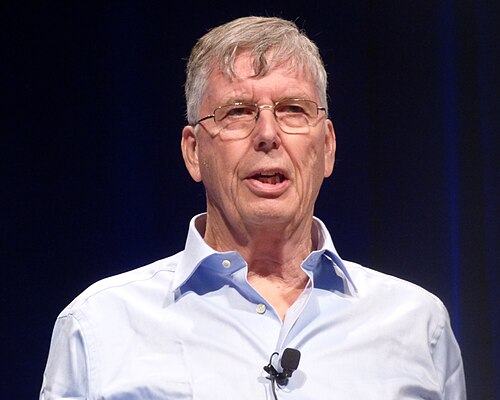
\includegraphics[width=1.80cm,height=2.20cm,keepaspectratio]{images/michaelstonebraker.jpg}
      };
      \node[inner sep=0pt] at (0.00,0) {
        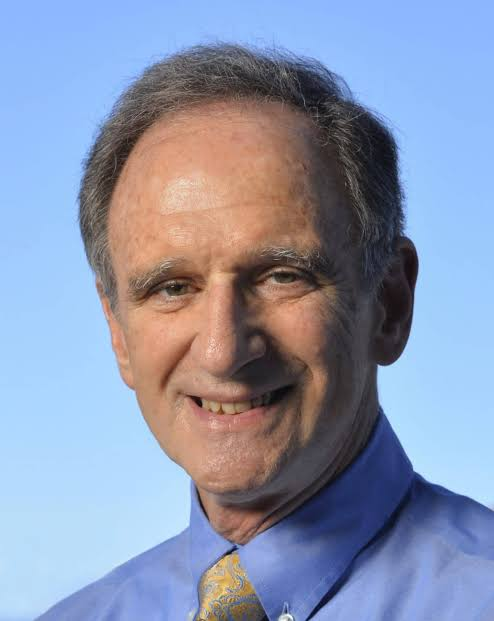
\includegraphics[width=1.80cm,height=2.20cm,keepaspectratio]{images/martinhellman.jpg}
      };
      \node[inner sep=0pt] at (1.50,0) {
        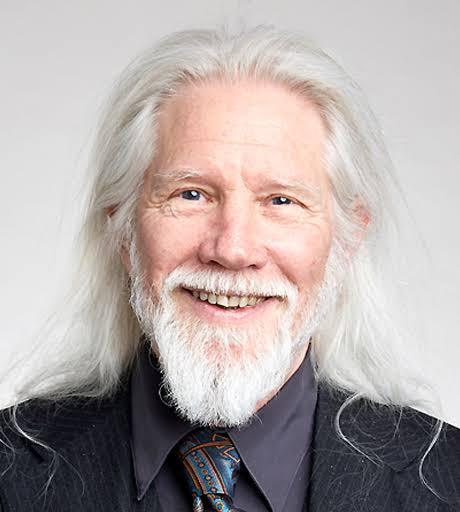
\includegraphics[width=1.80cm,height=2.20cm,keepaspectratio]{images/whitfielddiffie.jpg}
      };
      \node[inner sep=0pt] at (3.00,0) {
        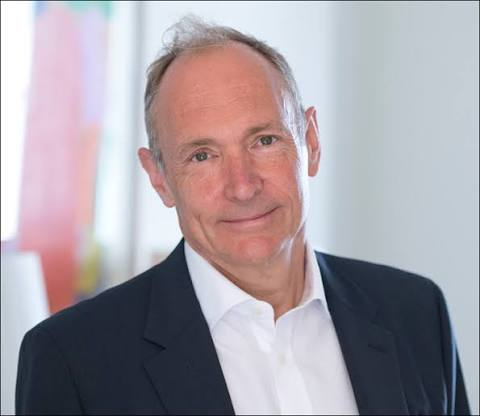
\includegraphics[width=1.80cm,height=2.20cm,keepaspectratio]{images/timbernerslee.jpg}
      };
  \end{tikzpicture}}
\end{frame}


\def\framesubject{RISC、RAID·RISC 体系结构·深度学习三杰之一·深度学习三杰之一·深度学习三杰之一}
\begin{frame}{2017–2018}
\vspace{-2pt}
\centering
\scriptsize
\begin{tabular}{@{}
  >{\raggedright}m{2.5cm}
  >{\centering}m{1.0cm}
  >{\centering}m{1.95cm}
  >{\raggedleft}m{1.5cm}
  >{\raggedright}m{2.2cm}
  >{\raggedright\arraybackslash}m{2.35cm}
@{}}
\toprule
\rowcolor{turingbg}
\textbf{姓名} & \textbf{获奖年份} & \textbf{生卒} & \textbf{国籍} & \textbf{机构} & \textbf{研究领域} \\
\midrule
  \lrow{David Patterson\cn{大卫·帕特森}}{2017}{1947–}{美国}{UC Berkeley}{RISC、RAID，与 Hennessy 共同奠基现代体系结构。}
  \lrow{John L. Hennessy\cn{约翰·亨尼西}}{2017}{1952–}{美国}{Stanford University}{RISC 体系结构，计算机体系结构教科书作者。}
  \lrow{Geoffrey Hinton\nobelbadge\frsbadge\cn{杰弗里·辛顿}}{2018}{1947–}{英国/加拿大}{University of Toronto}{深度学习三杰之一，反向传播、神经网络复兴。}
  \lrow{Yann LeCun\nsmbadge\nasbadge\cn{杨立昆}}{2018}{1960–}{法国/美国}{New York University}{深度学习三杰之一，卷积神经网络（CNN）之父。}
  \lrow{Yoshua Bengio\frsbadge\cn{约书亚·本吉奥}}{2018}{1964–}{加拿大/法国}{Université de Montréal}{深度学习三杰之一，表示学习与生成模型。}
\bottomrule
\end{tabular}
\vspace{6pt}
  {\centering
  \begin{tikzpicture}
      \node[inner sep=0pt] at (-3.00,0) {
        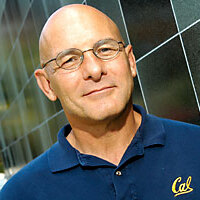
\includegraphics[width=1.80cm,height=2.20cm,keepaspectratio]{images/davidpatterson.jpg}
      };
      \node[inner sep=0pt] at (-1.50,0) {
        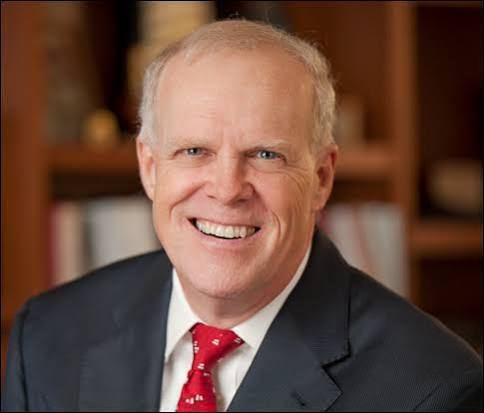
\includegraphics[width=1.80cm,height=2.20cm,keepaspectratio]{images/johnlhennessy.jpg}
      };
      \node[inner sep=0pt] at (0.00,0) {
        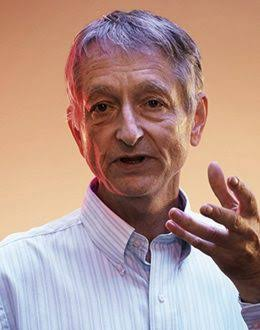
\includegraphics[width=1.80cm,height=2.20cm,keepaspectratio]{images/geoffreyhinton.jpg}
      };
      \node[inner sep=0pt] at (1.50,0) {
        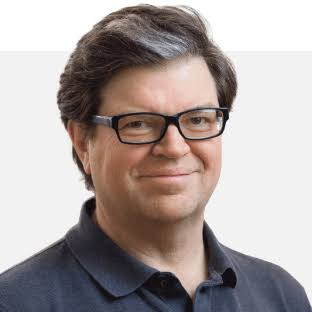
\includegraphics[width=1.80cm,height=2.20cm,keepaspectratio]{images/yannlecun.jpg}
      };
      \node[inner sep=0pt] at (3.00,0) {
        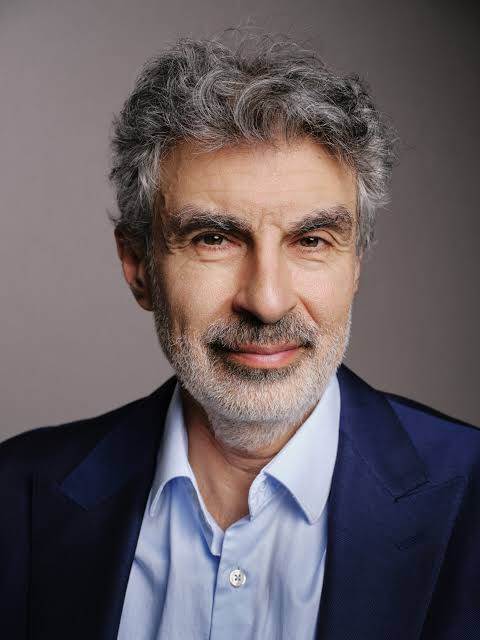
\includegraphics[width=1.80cm,height=2.20cm,keepaspectratio]{images/yoshuabengio.jpg}
      };
  \end{tikzpicture}}
\end{frame}


\def\framesubject{计算机图形学、纹理映射、皮克·RenderMan 渲染系统·编译器理论、《龙书》合著者。·编译、数据库、数据挖掘、《龙·LINPACK/LAPACK}
\begin{frame}{2019–2021}
\vspace{-2pt}
\centering
\scriptsize
\begin{tabular}{@{}
  >{\raggedright}m{2.5cm}
  >{\centering}m{1.0cm}
  >{\centering}m{1.95cm}
  >{\raggedleft}m{1.5cm}
  >{\raggedright}m{2.2cm}
  >{\raggedright\arraybackslash}m{2.35cm}
@{}}
\toprule
\rowcolor{turingbg}
\textbf{姓名} & \textbf{获奖年份} & \textbf{生卒} & \textbf{国籍} & \textbf{机构} & \textbf{研究领域} \\
\midrule
  \lrow{Edwin Catmull\cn{埃德温·卡特穆尔}}{2019}{1945–}{美国}{Pixar}{计算机图形学、纹理映射、皮克斯联合创始人。}
  \lrow{Pat Hanrahan\cn{帕特·汉拉汉}}{2019}{1955–}{美国}{Stanford University}{RenderMan 渲染系统、图形着色语言。}
  \lrow{Alfred Aho\cn{阿尔弗雷德·阿霍}}{2020}{1941–}{美国}{Columbia University}{编译器理论、《龙书》合著者。}
  \lrow{Jeffrey Ullman\cn{杰弗里·乌尔曼}}{2020}{1942–}{美国}{Stanford University}{编译、数据库、数据挖掘、《龙书》合著者。}
  \lrow{Jack Dongarra\nsmbadge\frsbadge\cn{杰克·唐加拉}}{2021}{1950–}{美国}{University of Tennessee}{LINPACK/LAPACK、MPI，高性能计算奠基人。}
\bottomrule
\end{tabular}
\vspace{6pt}
  {\centering
  \begin{tikzpicture}
      \node[inner sep=0pt] at (-3.00,0) {
        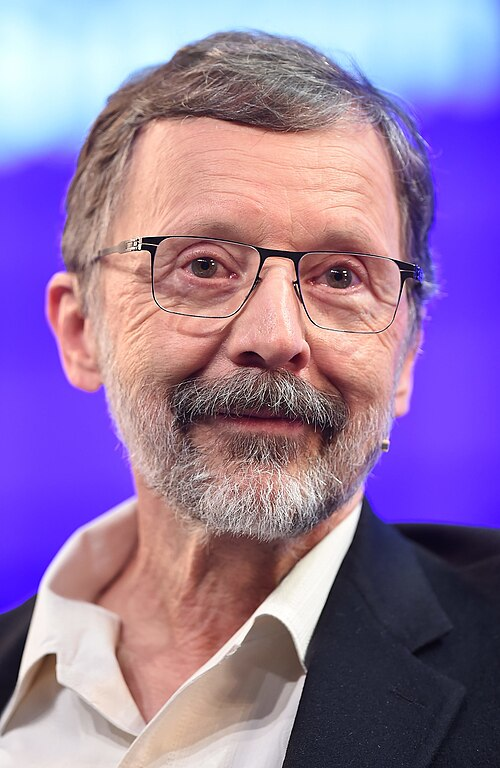
\includegraphics[width=1.80cm,height=2.20cm,keepaspectratio]{images/edwincatmull.jpg}
      };
      \node[inner sep=0pt] at (-1.50,0) {
        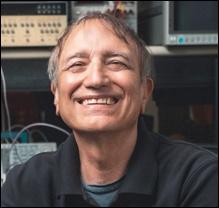
\includegraphics[width=1.80cm,height=2.20cm,keepaspectratio]{images/pathanrahan.jpg}
      };
      \node[inner sep=0pt] at (0.00,0) {
        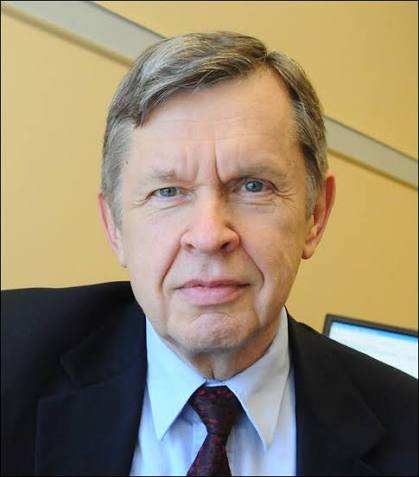
\includegraphics[width=1.80cm,height=2.20cm,keepaspectratio]{images/alfredaho.jpg}
      };
      \node[inner sep=0pt] at (1.50,0) {
        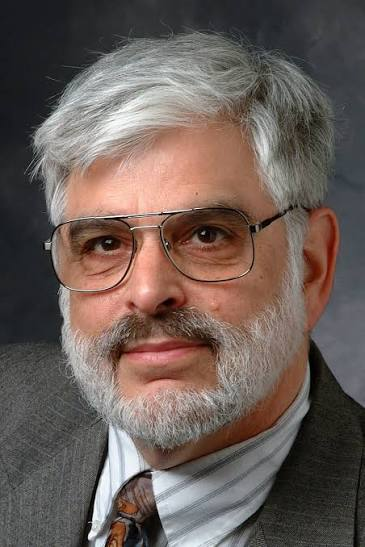
\includegraphics[width=1.80cm,height=2.20cm,keepaspectratio]{images/jeffreyullman.jpg}
      };
      \node[inner sep=0pt] at (3.00,0) {
        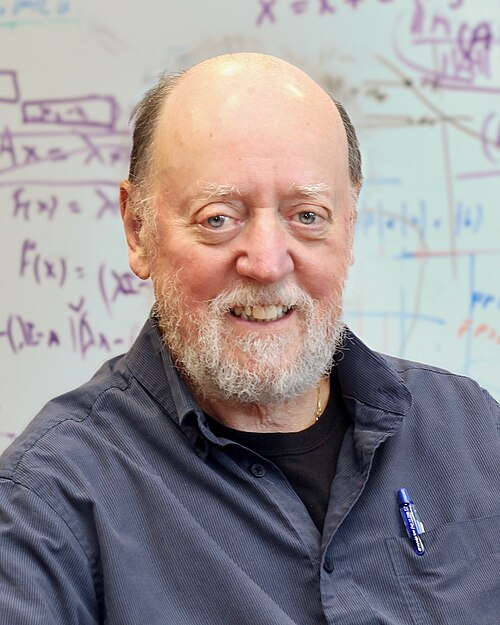
\includegraphics[width=1.80cm,height=2.20cm,keepaspectratio]{images/jackdongarra.jpg}
      };
  \end{tikzpicture}}
\end{frame}


\def\framesubject{以太网（Ethernet）发·随机性与计算、伪随机性与去随·强化学习奠基人·强化学习奠基人·量子信息科学、BB84 量子}
\begin{frame}{2022–2025}
\vspace{-2pt}
\centering
\scriptsize
\begin{tabular}{@{}
  >{\raggedright}m{2.5cm}
  >{\centering}m{1.0cm}
  >{\centering}m{1.95cm}
  >{\raggedleft}m{1.5cm}
  >{\raggedright}m{2.2cm}
  >{\raggedright\arraybackslash}m{2.35cm}
@{}}
\toprule
\rowcolor{turingbg}
\textbf{姓名} & \textbf{获奖年份} & \textbf{生卒} & \textbf{国籍} & \textbf{机构} & \textbf{研究领域} \\
\midrule
  \lrow{Robert Metcalfe\marconibadge\ntmbadge\cn{罗伯特·梅特卡夫}}{2022}{1946–}{美国}{MIT}{以太网（Ethernet）发明者，梅特卡夫定律。}
  \lrow{Avi Wigderson\godelbadge\abelbadge\nevanlinnabadge\cn{阿维·威格德森}}{2023}{1956–}{以色列/美国}{Institute for Advanced Study}{随机性与计算、伪随机性与去随机化，理论计算机巨星。}
  \lrow{Andrew Barto\cn{安德鲁·巴托}}{2024}{1948–}{美国}{University of Massachusetts}{强化学习奠基人，时间差分学习。}
  \lrow{Richard S. Sutton\cn{理查德·萨顿}}{2024}{1956–}{加拿大/美国}{University of Alberta}{强化学习奠基人，《强化学习导论》合著者。}
  \lrow{Charles H. Bennett\wolfbadge\shannonbadge\cn{查尔斯·贝内特}}{2025}{1943–}{美国}{IBM}{量子信息科学、BB84 量子密钥分发、可逆计算。}
\bottomrule
\end{tabular}
\vspace{6pt}
  {\centering
  \begin{tikzpicture}
      \node[inner sep=0pt] at (-3.00,0) {
        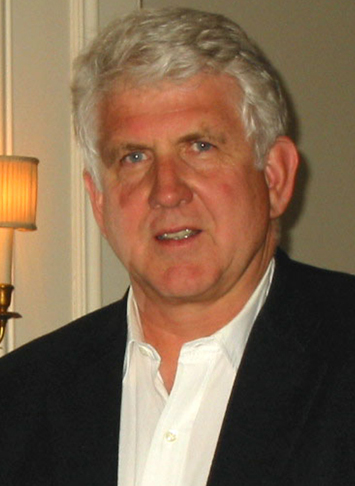
\includegraphics[width=1.80cm,height=2.20cm,keepaspectratio]{images/robertmetcalfe.jpg}
      };
      \node[inner sep=0pt] at (-1.50,0) {
        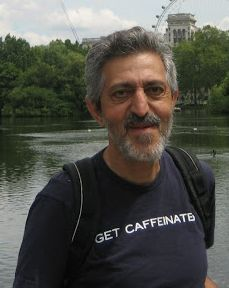
\includegraphics[width=1.80cm,height=2.20cm,keepaspectratio]{images/aviwigderson.jpg}
      };
      \node[inner sep=0pt] at (0.00,0) {
        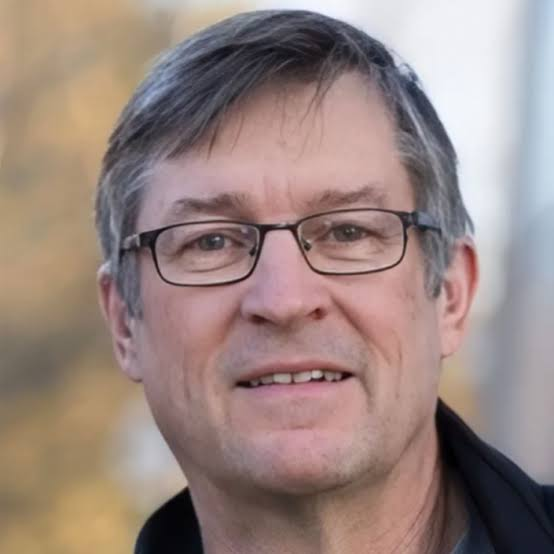
\includegraphics[width=1.80cm,height=2.20cm,keepaspectratio]{images/andrewbarto.jpg}
      };
      \node[inner sep=0pt] at (1.50,0) {
        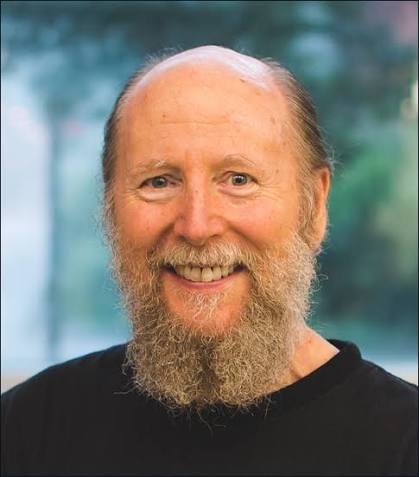
\includegraphics[width=1.80cm,height=2.20cm,keepaspectratio]{images/richardssutton.jpg}
      };
      \node[inner sep=0pt] at (3.00,0) {
        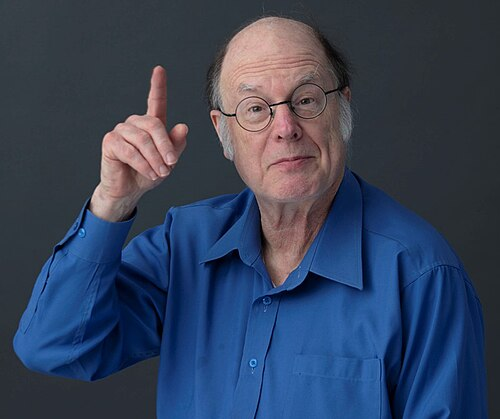
\includegraphics[width=1.80cm,height=2.20cm,keepaspectratio]{images/charleshbennett.jpg}
      };
  \end{tikzpicture}}
\end{frame}


\def\framesubject{量子密码学、BB84 协议、}
\begin{frame}{2025–2025}
\vspace{-2pt}
\centering
\scriptsize
\begin{tabular}{@{}
  >{\raggedright}m{2.5cm}
  >{\centering}m{1.0cm}
  >{\centering}m{1.95cm}
  >{\raggedleft}m{1.5cm}
  >{\raggedright}m{2.2cm}
  >{\raggedright\arraybackslash}m{2.35cm}
@{}}
\toprule
\rowcolor{turingbg}
\textbf{姓名} & \textbf{获奖年份} & \textbf{生卒} & \textbf{国籍} & \textbf{机构} & \textbf{研究领域} \\
\midrule
  \lrow{Gilles Brassard\wolfbadge\frsbadge\cn{吉勒·布拉萨}}{2025}{1955–}{加拿大}{Université de Montréal}{量子密码学、BB84 协议、量子纠缠理论。}
\bottomrule
\end{tabular}
\vspace{6pt}
  {\centering
  \begin{tikzpicture}
      \node[inner sep=0pt] at (-3.00,0) {
        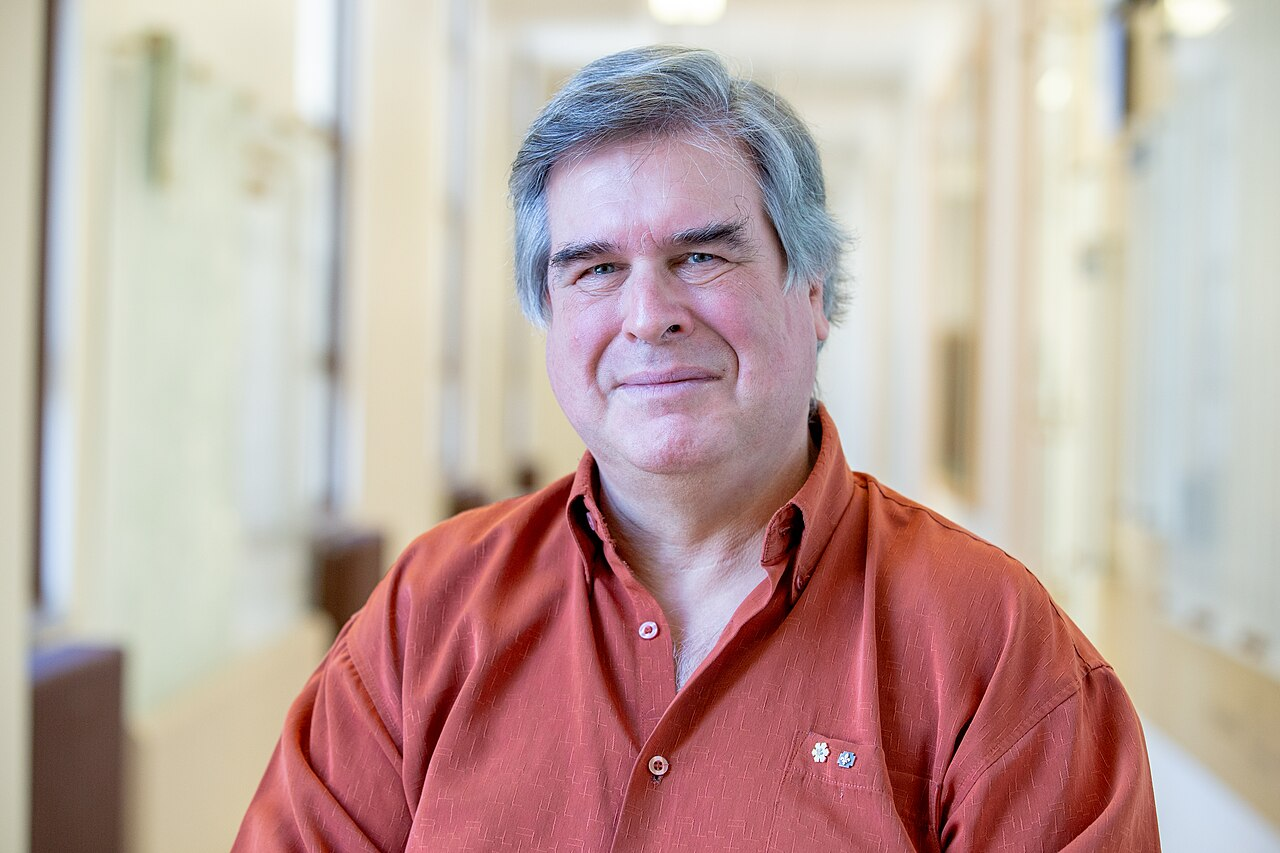
\includegraphics[width=1.80cm,height=2.20cm,keepaspectratio]{images/gillesbrassard.jpg}
      };
  \end{tikzpicture}}
\end{frame}


\end{document}
